\documentclass[french]{book}
\usepackage[utf8x]{inputenc}
\usepackage[T1]{fontenc}
\usepackage{babel}
\usepackage{lmodern}
\usepackage[top=2cm,bottom=2cm,left=3cm,right=3cm]{geometry}
\usepackage{microtype}
\usepackage{mathtools, amssymb, amsthm}
\usepackage{dsfont}
\usepackage{mdframed}
\usepackage{hyperref}
\usepackage{graphicx}
\usepackage{float}
\usepackage{xcolor}
\usepackage{mathrsfs}
\usepackage{wrapfig}
\usepackage{stmaryrd}
\usepackage{framed}
\usepackage{marginnote}
\usepackage[Glenn]{fncychap}


\newtheorem{prototheorem}{Théorème}[section]
\newenvironment{thm}
   {\colorlet{shadecolor}{orange!10}\begin{shaded}\begin{prototheorem}}
   {\end{prototheorem}\end{shaded}}

\newtheorem*{protocorollary}{Corollaire}
\newenvironment{corollary}
    {\colorlet{shadecolor}{violet!10}\begin{shaded}\begin{protocorollary}}
    {\end{protocorollary}\end{shaded}}

\newtheorem*{protolemma}{Lemme}
\newenvironment{lemma}
    {\colorlet{shadecolor}{pink!15}\begin{shaded}\begin{protolemma}}
    {\end{protolemma}\end{shaded}}

\theoremstyle{definition}
\newtheorem{protodefinition}{Définition}[section]
\newenvironment{definition}
    {\colorlet{shadecolor}{green!5}\begin{shaded}\begin{protodefinition}}
    {\end{protodefinition}\end{shaded}}

\newtheorem{protoproposition}{Proposition}[section]
\newenvironment{prop}
    {\colorlet{shadecolor}{blue!5}\begin{shaded}\begin{protoproposition}}
    {\end{protoproposition}\end{shaded}}

\theoremstyle{remark}
\newtheorem*{remark}{Remarque}
\newtheorem{exo}{Exercice}
\newtheorem*{protoexemple}{Exemple}
\newenvironment{exemple}
    {\colorlet{shadecolor}{gray!10}\begin{shaded}\begin{protoexemple}}
    {\end{protoexemple}\end{shaded}}

\newcommand{\lesss}{<}
\newcommand{\less}{\lesss}

\newcommand{\biggg}{>}
\newcommand{\bg}{\biggg}

\renewcommand\qedsymbol{$\clubsuit$}


\title{\bsc{Probabilités et applications}}
\author{Sandro \bsc{Vaienti}}
\date{2023-2024}

\begin{document}

\maketitle

\tableofcontents

\chapter{Généralités sur les probabilités}

\section{Tribus}


\begin{definition}[$\sigma$-algèbre $\mathscr{A} $]
  $\Omega$ ensemble. Les éléments de $\Omega$ constinuent une $\sigma$-algèbre $\mathscr{A} $ :

  \begin{enumerate}
    \item $\Omega \in \mathscr{A} $ ;
    \item Si $A \in \mathscr{A}  $, alors $A ^{C} \in \mathscr{A} $ ;
    \item Si $\{ A_n\} _{n=1} ^{\infty} $ est une suite dénombrable dans $\mathscr{A} $, alors $\bigcup_{n} A_n \in \mathscr{A}  $.
  \end{enumerate}

\end{definition}


\begin{exemple}

  \

  \begin{enumerate}
    \item $2 ^{\Omega}$, ensemble de tous les ensembles de $\Omega$, triviale ;
    \item Grossière $\{ \emptyset, \Omega \} $.
  \end{enumerate}
\end{exemple}



\begin{definition}[$\sigma$-algèbre engendrée]
  Dans $\Omega$, on a une famille d'ensembles $\mathscr{S} $. On appelle $\sigma(\mathscr{S} )$ la $\sigma$-algèbre engendrée par $\mathscr{S} $ qui est la plus petite $\sigma$-algèbre qui contient $\mathscr{S} $.

  \begin{equation*}
    \sigma(\mathscr{S} ) = \bigcap _{\substack {\mathscr{A} \sigma \text{ -algèbre } \\ \mathscr{A} _{\alpha} \in \mathscr{S}  }} \mathscr{A} _{\alpha}
  \end{equation*}
\end{definition}


\begin{exemple}
  $\Omega = \{ a,b,c \}, \mathscr{S} = \{ a, b \} $

  Construire $\sigma (\mathscr{S} )$.
\end{exemple}

\begin{exemple}
  $\Omega = \{ 1, 2, 3, 4 \} $ et $\mathscr{S} = \{ \{ 1 \}, \{ 2, 3 \} \} $. Construire $\sigma(\mathscr{S} )$.
\end{exemple}


\begin{exemple}
  On a dans $\Omega$ deux ensembles $A, B$. Construire $\sigma(\{ A, B \} )$.

  $\sigma(\{ A, B \} ) = \{ \Omega, \emptyset,A, B, A ^{C}, B ^{C}, A \cup B, A \cup B ^{C}, \dots \} $ (15 éléments).
\end{exemple}



\

Imaginons que $\Omega = \mathbb{R}$.

$\sigma$-algèbre de \bsc{Borel} ($\beta $). Il s'agit de la $\sigma$-algèbre engendrée par les intervalles ouverts.

$\mathscr{S} = \{ (a,b), (- \infty, a), (b, +\infty) \} $.

On a $[a, b) \in \beta $, car $\bigcap_{k=1} ^{\infty} (a - \frac{1}{k}, b) = [a,b)$.

\begin{remark}[intersections dans une $\sigma$-algèbre]
  Si $A, B \in \mathscr{A} $, est-ce que $A \cap B \in \mathscr{A} $ ?

  $A \cap B = (A ^{C} \cup B ^{C}) ^{C}$.

  $A -B = A \cap B ^{C}$. $A -B \in \mathscr{A} $.

  Les intersections dénombrables sont aussi dans $\mathscr{A} $.
\end{remark}

\begin{prop}
  $\beta $ est aussi engendrée par:
  \begin{enumerate}
    \item $\mathscr{S} _{1} = \{ [a,b) \} $ ;
    \item $\mathscr{S} _{2} = \{ (a,b] \} $ ;
    \item $\mathscr{S} _{3}  = \{ [a, +\infty) \} $ ;
    \item $\mathscr{S} _{4} = \{ (-\infty, a) \} $ ;
    \item $\mathscr{S} _{5} = \{ (a, +\infty) \} $.
  \end{enumerate}
\end{prop}

\begin{proof}
  On montre $\mathscr{S}_1 $.

  \begin{gather}
    [a,b) = \bigcap _{k=1} ^{\infty} \left(a- \frac{1}{k}, b\right) \implies \sigma([a,b)) \subset \beta .
  \end{gather}

  Montrons maintenant que $\beta  \in \sigma([a,b))$.

  \begin{equation*}
    \bigcup _{k=1} ^{\infty} \left[a+ \frac{1}{k}, b \right) = (a,b).
  \end{equation*}

  Donc $\beta \in \sigma([a,b))$.

  Montrons $\mathscr{S} _{3} $.
\end{proof}

\section{Probabilité}


\begin{definition}[Probabilité]
  Soit $(\Omega, \mathscr{A} )$ un espace mesurable.

  On introduit une fonction d'ensemble $\mathbb{P} : \mathscr{A} \longrightarrow [0, 1] $ qu'on appelle \textbf{probabilité} et qui vérifie :

  \begin{enumerate}
    \item $\mathbb{P}( \Omega ) = 1$ ;
    \item Si $(A_n)$ est une suite dénombrable dans $\mathscr{A} $ d'éléments deux à deux disjoints, alors

    \begin{equation*}
      \mathbb{P}\left( \bigcup _{n=1} ^{ \infty} A_n \right) = \sum_{n=1}^{\infty} \mathbb{P}( A_n ) .
    \end{equation*}
  \end{enumerate}
\end{definition}

Si $\{ A_n \} _{n=1} ^{\infty} $ est telle que $A_n$ ne sont pas deux à deux disjoints, alors

\begin{equation*}
  \mathbb{P}\left( \bigcup _{n=1} ^{\infty} A_n \right) \leq \sum_{n=1}^{\infty} \mathbb{P}( A_n ) .
\end{equation*}

Cette propriété s'appelle $\sigma$-sous additivité.

\subsection{Continuité}

Soit $\{ A_n \} $ une suite croissante, i. e. $A_n \subset A _{n+1}$.

Est-ce que

\begin{equation*}
  \mathbb{P}\left( \bigcup _{n=1} ^{\infty} A_n \right) = \lim_{n \to \infty} \mathbb{P}( A_n ) ?
\end{equation*}

Soit $\{ A_n \} _{n=1} ^{\infty} $ une suite décroissante, ie $A _{n+1} \subset A_n$, alors

\begin{equation*}
  \mathbb{P}\left( \bigcap _{n=1} ^{\infty}A_n \right) = \lim_{n \to \infty} \mathbb{P}( A_n ).
\end{equation*}

\begin{proof}
  \begin{equation*}
    \bigcup _{n=1} ^{\infty} A_n = A_1 \cup \left(\bigcup _{n=1} ^{\infty} (A _{n+1} \setminus A_n)\right)
  \end{equation*}

  \begin{figure}
    \centering
    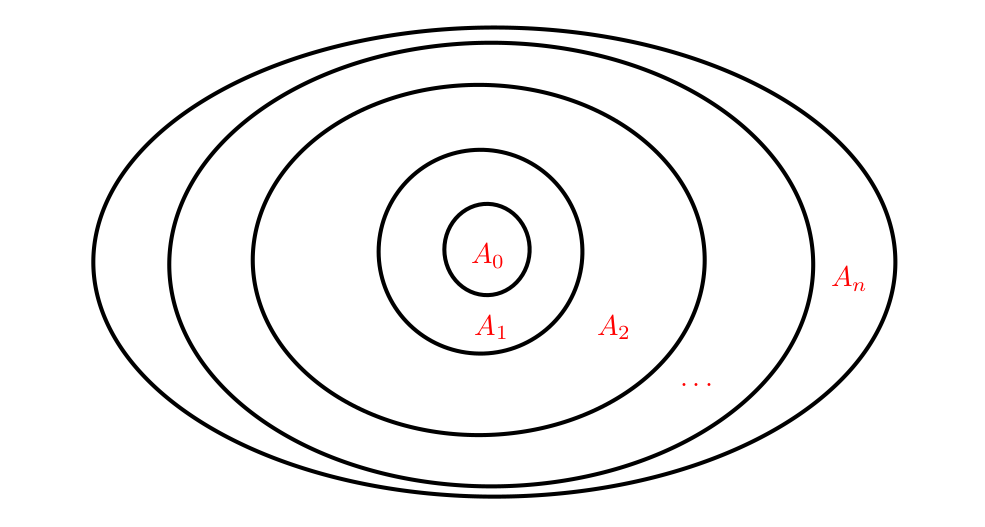
\includegraphics[scale=0.3]{figures/mesure-suite-ens.png}
    \caption{On construit ainsi les couronnes}
    \label{fig:mesure-suite-ens}
  \end{figure}


  Donc par le deuxième axiome, on a

  \begin{gather*}
    \mathbb{P}( \bigcup _{n=1} ^{\infty} A_n ) = \mathbb{P}( A_1 ) + \sum_{n=1}^{\infty} \mathbb{P}( A _{n+1} \setminus A_n ) \\
    = \mathbb{P}( A_1 ) + \lim_{k \to + \infty} \sum_{n=1}^{k} \mathbb{P}( A _{n+1} \setminus A_n ) \\
    =\mathbb{P}( A_1 ) + \lim_{k \to + \infty} \sum_{n=1}^{k} (\mathbb{P}( A _{n+1} ) - \mathbb{P}( A_n ) ) \text{ (somme téléscopique) }
  \end{gather*}

  Or on a

  \begin{gather*}
    \sum_{n=1}^{k} (\mathbb{P}( A _{n+1} ) - \mathbb{P}( A_n ) )  = \mathbb{P}( A _{k+1} ) - \mathbb{P}( A_1 ).
  \end{gather*}

  Donc

  \begin{gather*}
    \mathbb{P}\left( \bigcup _{n=1} ^{\infty} A_n \right) = \mathbb{P}( A_1 ) + \lim_{k \to \infty} [\mathbb{P}( A _{k+1} ) - \mathbb{P}( A_1 )]
  \end{gather*}

  et on obtient le résultat désiré.
\end{proof}

$(\Omega, \mathscr{A}, \mathbb{P} )$ espace mesuré ou de probabilité.

Dans le langage des probabilités, on appelle $\Omega$ l'univers et les éléments de $\mathscr{A} $ sont des événements.

\section{Mesure de Dirac}

Soit $\omega _{0} \in \Omega$ quelconque.

$\delta  _{w_0}(A), A \in \mathscr{A} $.

$\delta _{w_0}(A) =
 \begin{cases}
  1 \text{ si } w_0 \in A \\
  0 \text{ sinon}.
\end{cases}$

Montrer qu'il s'agit d'une probabilité.

\

 Soit $\Omega = \{ \omega_1, \omega_2, \dots, w_k, \dots \} $.

 On associe à $w_i$ un poids $p_i$ tel que

 \begin{equation}
   \sum_{i=1}^{\infty} p_i = 1.
 \end{equation}

 Si $A \subset \Omega$, on définit

 \begin{equation*}
   \mathbb{P}( A ) = \sum_{i,  \omega_i \in A}^{} p_i.
 \end{equation*}

 Si $card(\Omega) \less \infty$, $\Omega = \{ \omega_1, \omega_2, \dots, \omega _{N} \} $.

 On associe à $\omega _{j} = \frac{1}{N}$.

 Donc

 \begin{gather*}
   \mathbb{P}( A ) = \sum_{i, \omega_i \in A}^{} \frac{1}{N} = \frac{card(\omega_i \text{ dans } A)}{card(\text{total de } \omega_i )} = \frac{\text{ cas favorables } }{\text{ cas possibles } }.
 \end{gather*}

\section{Mesure de Lebesgue}

Elle est définie sur $\beta (\mathbb{R})$ et elle est la seule mesure qui se comporte comme ceci :

$\lambda ( (a,b] ) = b-a$.

On a aussi

\begin{equation}\label{lebesgue-zero}
  \lambda ((a,b)) = \lambda ([a,b]) = b-a.
\end{equation}

$(a,b] = (a,b) \cup \{ (b)\}$.

Il faut montrer que $\lambda (\{ b \} ) = 0$.

On a

\begin{gather*}
  \{ b \} = \bigcap _{n=1} ^{\infty} (b- \frac{1}{k}, b].
\end{gather*}

Donc

\begin{gather*}
  \lambda (\{ b \} ) = \lambda (\bigcap _{k=1} ^{\infty} (b - \frac{1}{k}, b]) \text{ intersection décroissante } \\
  = \lim_{k \to \infty} \lambda ((b- \frac{1}{k}, b]) \\
  = \lim_{k \to \infty} (b-b+ \frac{1}{k}) = \lim_{k \to \infty} \frac{1}{k} = 0.
\end{gather*}

\subsection{Mesure de Lebesgue-Stieltjes}

Soit $F$ une fonction croissante bornée et continue à droite (i. e. $F(x_0) = \lim_{x \to x_0} F(x)$) et supposons que

\begin{figure}[h!]
  \centering
  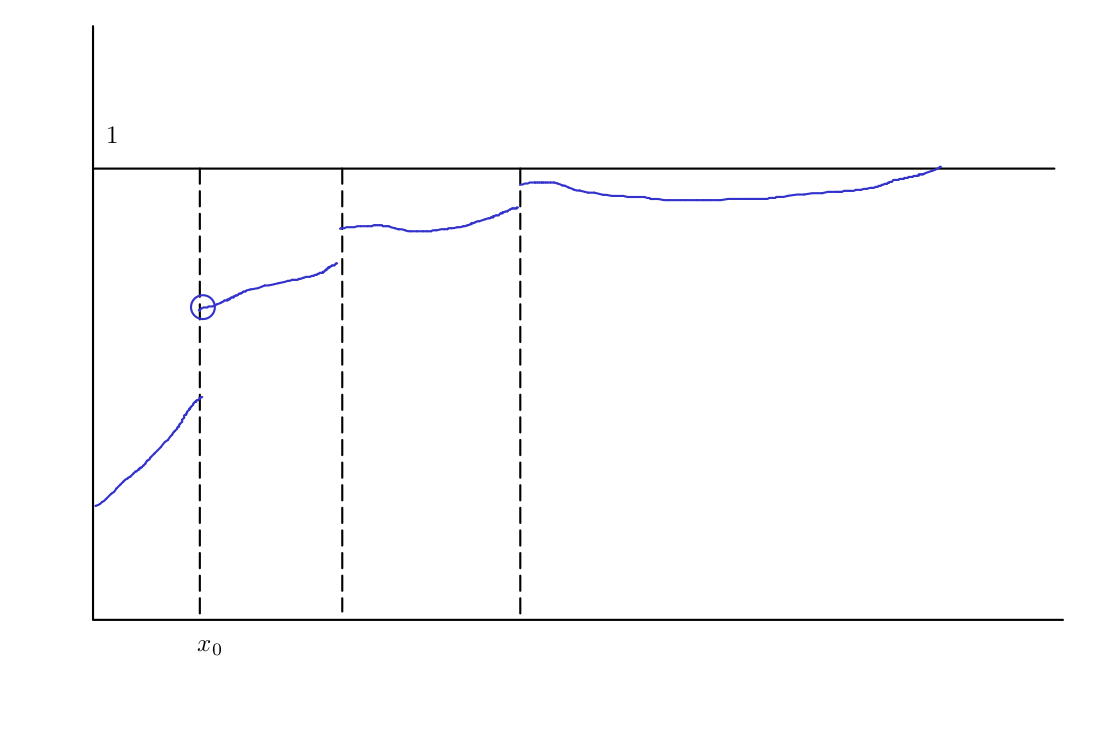
\includegraphics[scale=0.2]{figures/lebesgue-stieltjes}
  \caption{Mesure de Lebesgue-Stieltjes}
  \label{}
\end{figure}

On définit une fonction d'ensemble $\nu ((a,b]) = F(b) - F(a)$. $\nu$ devient une mesure de probabilité sur $\sigma((a,b]) = \beta $.

On a $\nu(\{ x_d \} ) \neq 0$.

\begin{proof}
  $\{ x_d \} = \bigcap_{k=1} ^{\infty} (x_d - \frac{1}{k}, x_d] $.

  Or
  \begin{gather*}
    \nu(\{ x_d \} ) = \lim_{k \to \infty} \nu((x_d - \frac{1}{k}, x_d]) = \lim_{k \to \infty} F(x_d) - F(x_d - \frac{1}{k}) \\
    = F(x_d) - \lim_{k \to \infty} F(x_d - \frac{1}{k})  = F(x_d) _{+} - F(x_d) _{-} \\
    = \text{ différence entre la limite gauche et la limite droite } \bg 0.
  \end{gather*}
\end{proof}

\section{Fonctions mesurables}

$(\Omega, \mathscr{A} ) \to (\mathbb{R}, \beta )$, $f : \Omega \to \mathbb{R}$.

\begin{definition}[Mesurable]
  On dit que $f$ est mesurable si pour tout borélien $B \in \beta $, $f ^{-1} (B) \in \mathscr{A} $.
\end{definition}

\begin{definition}[Equivalente]
  $f ^{-1} (\beta )$ est une sous $\sigma$-algèbre de $\mathscr{A} $.
\end{definition}

\begin{exo}
  Montrer que $f ^{-1} (\beta )$ est une $\sigma$-algèbre.
\end{exo}

\begin{proof}
  \begin{enumerate}
    \item $f ^{-1} (\mathbb{R}) = \Omega$.
    \item Si $A \in f ^{-1} (\beta )$, est-ce que $A ^{C}$ est aussi dans $f ^{-1} (\beta )$ ?

    Si $A \in f ^{-1} (\beta )$, alors $\exists B \in \beta $ tel que $A = f ^{-1} (B)$.

    $A ^{C} = (f ^{-1} (B)) ^{C} = f ^{-1} (B ^{C})$.

    \item Si $\{ A_n \} \in f ^{-1} (\beta ) $, est-ce que $\bigcup_{n=1} ^{\infty} A_n \in f ^{-1} (\beta ) $ ?
  \end{enumerate}
\end{proof}

\begin{prop}
  $f : \Omega \to \mathbb{R}$.

  Soit $\mathscr{C} $ une famille dans $\mathbb{R}$ telle que $\sigma(\mathscr{C} ) = \beta $.

  Si $ f ^{-1} (C ) , C \in \mathscr{C} $ est dans $\mathscr{A} $, alors $f$ est mesurable.
\end{prop}

\begin{exemple}
  $f : \Omega \text{ (topologie) }  \longrightarrow \mathbb{R} \text{ (topologie ouverts) } $ continue.

  $f$ est mesurable.

  Si $\mathcal{O}$ ouvert dans $\mathbb{R}$, $f ^{-1} (\mathcal{O})$ est ouvert dans $\Omega$.
\end{exemple}

\

$f : (\Omega, \mathscr{A} ) \longrightarrow (\mathbb{R}, \beta )$. Pour tout $\omega \in \Omega$, $f(\omega) = \text{ constante. } $

On a deux cas :

\begin{enumerate}
  \item $f ^{-1} ((a,b)) = \emptyset$ si la constante n'est pas dans $(a,b)$;
  \item $f ^{-1} ((a,b)) = \Omega$ si la constante est bien dans $(a,b)$.
\end{enumerate}

\begin{exemple}
  Soient $f, g : (\Omega, \mathscr{A} ) \to (\mathbb{R}, \beta )$ deux fonctions mesurables. Montrons que $f+g$ est mesurable.
\end{exemple}


\begin{proof}
  On considère la famille $\{ (a, \infty) \}$.

  Si on veut montrer que $f+g$ est mesurable, il suffit de montrer que $(f+g) ^{-1} ((a, \infty)) \in \mathscr{A} $.

  Donc il faut montrer que $\{ \omega, f(\omega) + g(\omega) \bg a \} \in \mathscr{A}  $, ie $\{ \omega, f(\omega) \bg a - g(\omega) \} $.

  Montrons d'abord que $a - g$ est mesurable.

  $\omega \in (a - g) ^{-1} ((b, \infty))$.

  \begin{gather*}
    a - g(\omega) \bg b \implies - g(\omega) \bg b-a \\
    \text{Or }\{ \omega, g(\omega) \less a-b \} \in \mathscr{A}, \\
    \text{c'est à dire } g ^{-1} ((- \infty, a-b)) \in \mathscr{A} .
  \end{gather*}

  Notons $h = a - g$.

  Si $f, h$ sont mesurables, est-ce que $\{ \omega, f(\omega) \bg h(w) \} $ ?

  On a $\{ \omega, f(\omega) \bg h(x) \} = \bigcup_{r \in \mathbb{Q}} \{ f \bg r \} \cap \{ h \less r \} $.

  Or $\{ \omega, f(\omega) \bg r \} = f ^{-1} (r, \infty)  \in \mathscr{A} $ et $\{ \omega, h (\omega) \less r \} = h ^{-1} ((-\infty, r)) \in \mathscr{A}  $.

  On a donc montré que $f+g$ est mesurable.
\end{proof}

\begin{prop}
  On a aussi :
  \begin{enumerate}
    \item Si $\lambda $ est un scalaire, $\lambda f$ est mesurable ;
    \item $f \cdot g$ est mesurable ;
    \item Si $g \neq 0$, $\frac{f}{g}$ est mesurable ;
    \item Si on a une suite $\{ f_n \} _{n \in \mathbb{N}} $ de fonctions mesurables, on a $\sup f_n, \inf f_n, \lim \sup f_n, \lim \inf f_n$ sont mesurables.
  \end{enumerate}
\end{prop}

Soient $\Omega \in \mathbb{R}$ borné et $f : (\Omega, \beta ) \longrightarrow (\mathbb{R}, \beta )$.

Soit $\mathcal{P}$ une partition de $\Omega$, ie un ensemble $\mathcal{P} = \{ P_i \} _{i=1} ^{\infty} $ tel que $$\bigcup_{i=1} ^{\infty} P_i = \Omega \text{ et } P_i \cap P_j \neq 0 \text{ si } i \neq j. $$

Considérons par exemple la partition $\mathcal{P} = \{ P_1, P_2, P_3, P_4 \} $.

Comme $\mathcal{P}$ est une famille dans $\Omega$, construisons $\sigma(\mathcal{P})$, ie la $\sigma$-algèbre engendrée par $\mathcal{P}$.  Dans notre cas, $\sigma(P_1, P_2, P_3, P_4)$.

Cette $\sigma$-algèbre est composée par la réunion d'éléments de $\mathcal{P} \cup \{ \emptyset \}$.

\begin{gather*}
  \sigma(\mathcal{P}) = \{ \emptyset, \Omega, P_1, P_2, P_3, P_4, P_1 ^{C} = P_2 \cup P_3 \cup P_4, \dots  \}.
\end{gather*}

Si on a $B = \bigcup_{i=1} ^{m} P_i $, alors $B ^{C} = \bigcap_{i=1} ^{m} P_i ^{C} = \bigcap_{i=1}^{m} \left(\bigcup_{i=1}^{m} P_i\right)   $.

\begin{prop}
  On sait exactement comment sont faites les fonctions mesurables dans ce cas. Il s'agit de fonctions constantes par morceaux.
\end{prop}

\begin{proof}
  Soit $ \{ p \} \in \mathbb{R}$, donc $f ^{-1} (\{ p \} ) \in \sigma(\mathcal{P})$.

  Supposons par exemple que $f ^{-1} (\{ p \} ) = P_2 \cap P_3$. Si $x \in f ^{-1} (\{ p \} )$, alors $ f(x) = p$, mais $x \in P_2 \cup P_3$, donc sur $P_2 \cup  P_3$ on aura en fait une valeur constante.

   %donc si $x \in f ^{-1} (\{ p \} ), f(x)=p, x \in P_2 \cup P_3$.
\end{proof}

\

\begin{definition}[Variable aléatoire]
  Soit $X : (\Omega, \mathscr{A}, \mathbb{P} ) \longrightarrow (\mathbb{R}, \beta )$.

  Si $X$ est une fonction mesurable, on dit que $X$ est une \textbf{variable aléatoire}.
\end{definition}

\begin{remark}[Notations]
  On notera

  $$\mathbb{P}( X \in B ) = \mathbb{P}( \omega, X(\omega) \in B ). $$

\end{remark}



\section{Loi de la variable aléatoire}

\begin{definition}[Loi de variable aléatoire]\label{loi_va}
  Il s'agit d'une mesure de probabilité définie sur $\mathbb{R}$. On va la noter avec le symbole $P_X$.

  Si $B \in \beta $, $$P_X(B) = \mathbb{P}( X ^{-1} (B) ),$$ avec $$X ^{-1} (B) = \{ \omega \mid X(\omega) \in B \}.$$
\end{definition}



\begin{definition}[Rappel : mesure (cf cours d'intégration de L3)]

  \

  Soit $(E, \tau)$ un ensemble mesurable. Alors une application $\mu : \tau \to \overline{\mathbb{R} ^{+}} $ est une mesure sur $E$ si :
 \begin{enumerate}
   \item $\mu(\emptyset) = 0$;
   \item Pour toute suite $(A_n)$ de $\tau$ disjointe, ie $A_n \cap A_m = \emptyset$ si $m \neq n$, alors $$\mu \left(\bigcup_{n \in \mathbb{N}} A_n \right) = \sum_{n \in \mathbb{N}} \mu(A_n) \ (\sigma \text{-additivité.})$$
 \end{enumerate}
\end{definition}

\begin{figure}[h!]
  \centering
  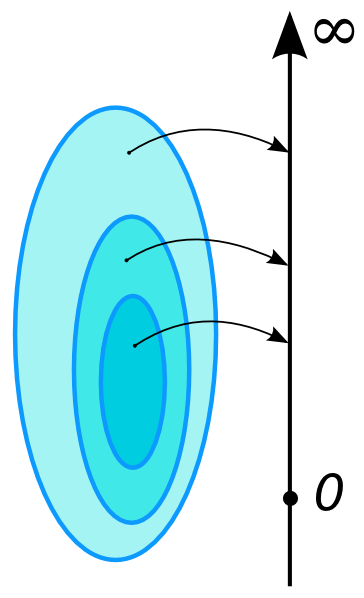
\includegraphics[scale=0.3]{figures/Measure_illustration.png}
  \caption{De façon informelle, une mesure a la propriété d'être monotone : si l'ensemble $ E$ est un sous-ensemble de $ F$, la mesure de $ E$ est inférieure ou égale à celle de $ F$. De plus, on impose à la mesure de l'ensemble vide la valeur 0 (Wikipédia).}
  \label{}
\end{figure}

\begin{exo}
  Montrer que $P_X$ est une mesure.
\end{exo}

\begin{proof}
  \begin{enumerate}
    \item $P_X(\mathbb{R}) = \mathbb{P}( X ^{-1} (\mathbb{R}) ) = \mathbb{P}( \Omega ) = 1$ ;
    \item Si $\{ B_n \} $ est une suite deux à deux disjointe,

    \begin{gather*}
      P_X \left( \bigcup _{n=1} ^{\infty} B_n \right) = \sum_{n=1}^{\infty} P_X(B_n),
    \end{gather*}

    car

    \begin{gather*}
      P_X \left(\bigcup _{n=1} ^{\infty} B_n \right) = \mathbb{P}\left( X ^{-1} \left(\bigcup _{n=1} ^{\infty} B_n \right) \right) \\
      = \mathbb{P} \left( \bigcup _{n=1} ^{\infty} X ^{-1} (B_n) \right) \text{ (propriété de l'image réciproque) }  \\
      = \sum_{n=1}^{\infty} \mathbb{P}( X ^{-1} (B_n) ) \ (\mathbb{P} \text{ est une probabilité} ) \\
      = \sum_{n=1}^{\infty} P_X (B_n).
    \end{gather*}
  \end{enumerate}
\end{proof}

\marginnote{15-09-2023}

\section{Intégrale}

\begin{definition}[Fonctions étagées/simples]
  Soit $X$ espace mesuré, $x \in X$. Une fonction $h$ est appelée fonction étagée si $h$ s'écrit de la manière suivante

  $$ h(x) = \sum_{k=1}^{M} c_k \mathds{1} _{A_k}(x), $$

  avec $A_k$ ensemble mesurables (un élément de la $\sigma$-algèbre) tel que $A_k \cap A_j$ si $k \neq j$ et $c_k \geq 0$.


\end{definition}

\begin{thm}
  Soit $f : (X, \mathscr{A}, \mu )$ (espace mesuré) $\longrightarrow (\mathbb{R} ^{+}, \beta )$ mesurable.

  Alors il existe une suite croissante $(\forall x, h_n(x) \leq h _{n+1}(x))$ de fonctions étagées  $\{ h_k \} _{n \in \mathbb{N}}$ telle que

  \begin{gather*}
    f(x) = \lim_{n \to \infty} h_n(x).
  \end{gather*}
\end{thm}

\begin{definition}[Intégrale de Lebesgue]

  \

  \begin{enumerate}
    \item \emph{Première étape.} On considère une fonction simples

    $$ h(x) = \sum_{k=1}^{M} c_k \mathds{1} _{A_k}(x), $$

    alors $$ \int_{X}^{} h d \mu = \int_{X}^{}h(x) d \mu(x) = \sum_{k=1}^{M} c_k \mu(A_k).$$

    \item \emph{Deuxième étape.} Si $f$ est mesurable non négative,

    \begin{enumerate}
      \item $$ \int_{X}^{} f d \mu = \sup \left( \int_{X}^{} h d \mu, h \text{ simple, } h \leq f \right). $$
      \item Si $f = \lim_{k \to \infty} h_k, h_k $ simples non négatives,

      $$ \int_{X}^{} f d \mu = \lim_{k \to \infty} \int_{}^{} h_k d \mu.$$
    \end{enumerate}

    \item Si $f$ mesurable de signe quelconque, on écrit $f(x) = f _{+}(x) - f _{-}(x)$, où $f _{+} = \max (f,0)$ et $f _{-} = \max (-f, 0)$.

    (à suivre...)

  \end{enumerate}
\end{definition}

\begin{definition}[De classe $\mathscr{L} ^{1}$]
  On dira que $f$ est de classe $\mathscr{L} ^{1} $ si

  $$ \int_{X}^{} \lvert f \rvert d \mu \less +\infty. $$

  Dans ce cas, $\lvert f \rvert = f _{+} + f _{-}$.
\end{definition}


\begin{exemple}
  On considère la mesure de Dirac

  %\begin{figure}[h!]
  %  \centering
  %  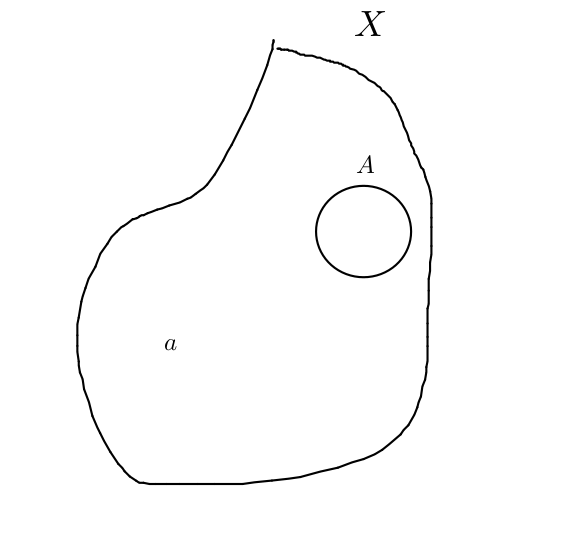
\includegraphics[scale=0.3]{figures/L1.png}
  %  \caption{}
  %  \label{}
  %\end{figure}

  $$ \delta _a (A) = \begin{cases}
    1 \text{ si } a \in A \\
    0 \text{ sinon. }
  \end{cases}$$

  Alors \begin{equation}\label{int_dirac}
     \int_{X} f(x) d \delta _a(x) = f(a) .
  \end{equation}
\end{exemple}



\begin{proof}
  Soit $f = \sum_{k=1}^{M} c_k \mathds{1} _{A_k}$ une fonction simple.

  \begin{gather*}
    \int_{}^{} \sum_{k=1}^{M} c_k \mathds{1} _{A_k}(x) d \delta _a(x) = \sum_{k=1}^{M} c_k \delta _a(A_k) = c _{\overline{k} } \\
     \text{ avec } \overline{k} \text{ le seul } k \text{ tel que } a \in A _{k } \text{ car les } A_k \text{ sont deux à deux disjoints. }
  \end{gather*}

  Or $c _{\overline{k} } = f(a)$.

  \begin{figure}[h!]
    \centering
    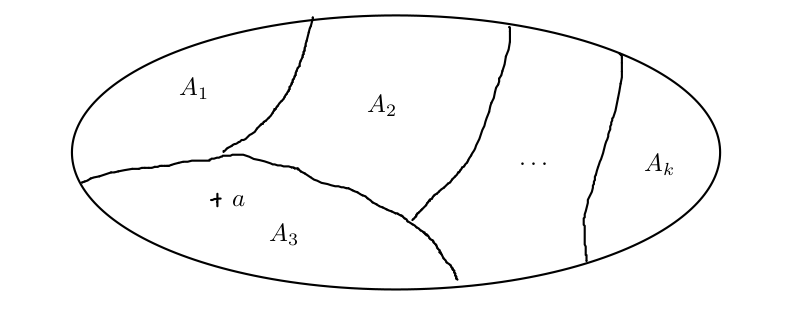
\includegraphics[scale=0.3]{figures/fct_etagees_ak.png}
    \caption{$a$ ne peut être que dans un seul des $A_k$.}
    \label{}
  \end{figure}

  \

  On suppose maintenant que $f(x) = \lim_{k \to \infty} h_k(x) $.

  Alors

  \begin{gather*}
    \int_{X}^{} f(x)d \delta _a(x) = \int_{X}^{} \lim_{k \to \infty}h_k(x) d \delta _a(x) \stackrel{\text{Beppo-Levi}}{=} \lim_{k \to \infty} \int_{X}^{} h_k d \delta _a(x) = \lim_{k \to \infty} h_k(a)= f(a).
  \end{gather*}
\end{proof}

\begin{thm}[Beppo-Levi]
  Si $\{ h_k \} $ est une suite monotone non négative, alors

  $$ \lim \int f_k = \int_{}^{} \lim_{ } f_k.$$
\end{thm}

\begin{remark}
  Si $\mu = \sum_{k=1}^{M} p_k \delta _{a_k} $, avec $\sum_{k=1}^{M} p_k = 1 $, alors

  $$ \int_{X}^{} f d \left(\sum_{k=1}^{M} p_k \delta _{a_k}  \right) = \sum_{k=1}^{M} p_k f(a_k).$$
\end{remark}

\begin{proof}
  Même démonstration que pour \ref{int_dirac}.
\end{proof}

\subsection{Conséquences en probabilités}


Soit $X : (\Omega, \mathscr{A}, \mathbb{P} ) \longrightarrow (\mathbb{R}, \beta)$.

$X$ est une variable aléatoire. Associée à $X$, il y a une mesure de Borel sur la droite qu'on appelle la loi notée $P_X$ (cf \ref{loi_va}).

\begin{definition}[Espérance de $X$]
  L'espérance de $X$ se calcule comme suit :

  \begin{equation}
    \mathbb{E}[ X ] = \int_{\Omega}^{} X(\omega) d \mathbb{P}( \omega ).
  \end{equation}
\end{definition}

\begin{thm}[De transfert]
  On a

  \begin{equation}
    \int_{\Omega}^{} f(X(\omega)) d \mathbb{P}( \omega ) = \int_{\mathbb{R}}^{} f(x) d P_X(x), \text{ avec } x \in \mathbb{R}.
  \end{equation}
\end{thm}

\begin{proof}
  Soit $f : \mathbb{R} \to \mathbb{R}$ fonction simple telle que $f(x) = \sum_{k=1}^{M} c_k \mathds{1} _{A_k}(x) $.

    \begin{figure}[h!]
      \centering
      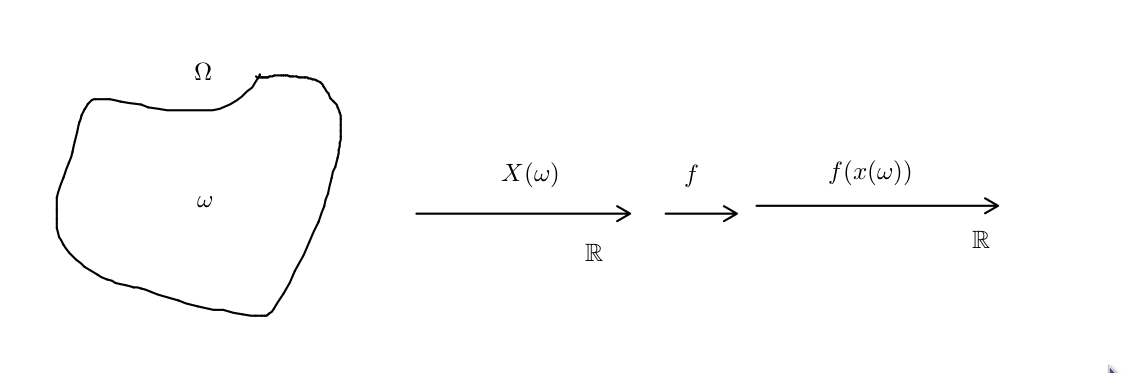
\includegraphics[scale=0.3]{figures/transfert.png}
      \caption{Illustration théorème de transfert}
      \label{}
    \end{figure}

  \begin{gather}\label{transfert-1}
    \int_{\Omega}^{} \sum_{k=1}^{M} c_k \mathds{1} _{A_k}(X (\omega)) d \mathbb{P}( \omega )  = \sum_{k=1}^{M} c_k \int_{\Omega}^{} \mathds{1} _{A_k}(X(\omega)) d \mathbb{P}( \omega ).
  \end{gather}

  Or

  \begin{gather*}
    \int_{\Omega}^{} \mathds{1} _{A_k}(X (\omega)) d \mathbb{P}( \omega ) = \int_{\Omega}^{} \mathds{1} _{X ^{-1} (A_k)}(\omega) d \mathbb{P}( \omega ) = \mathbb{P}( X ^{-1} (A_k) ) = P_X (A_k)
  \end{gather*}

  Donc \ref{transfert-1} devient :

  \begin{gather*}
    \sum_{k=1}^{M} c_k P_X(A_k) = \int_{\mathbb{R}}^{} f(x) d P_X(x).
  \end{gather*}

  \

  On considère que $f$ est quelconque avec $f = \lim_{k \to \infty} h_k$, avec $\{ h_k \} $ suite de fonctions simples.

  \begin{gather*}
    \int_{}^{} f(X(\omega)) d \mathbb{P}( \omega ) = \int_{}^{} \lim_{k \to \infty}   h_k(X(\omega)) d \mathbb{P}( \omega ) = \lim_{k \to \infty} \int_{}^{} h_k (X(\omega)) d \mathbb{P}( \omega ) \\
    =\lim_{k \to \infty} \int_{\mathbb{R}}^{} h_k(x) d P_X(x) =  \int_{\mathbb{R}}^{} \lim_{k \to \infty} h_k(x) d P_X(x) = \int_{\mathbb{R}}^{} f d P_X
  \end{gather*}

\end{proof}

\section{Fonctions de répartition}

\begin{definition}[Fonction de répartition]
  Soit $X : \Omega \longrightarrow \mathbb{R}$ une variable aléatoire. On définit

  \begin{gather}
    F(t) = \mathbb{P}( X \leq t ), t \in \mathbb{R} \\
    = \mathbb{P}( \omega, X(\omega) \leq t ) = \mathbb{P}( X ^{-1} ((-\infty, t]) ) = P_X((-\infty, t]).
  \end{gather}
\end{definition}



\begin{figure}[h!]
  \centering
  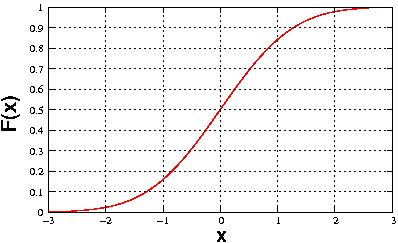
\includegraphics[scale=0.5]{figures/F_repartition.png}
  \caption{Fonction de répartition}
  \label{}
\end{figure}

\begin{prop}[Propriétés de $F$]

  \

  \begin{enumerate}
    \item $F$ est non négative et bornée entre 0 et 1.
    \item $F$ est croissante et continue à droite.
    \item $$ \begin{cases}
      \lim_{t \to +\infty} F(t) = 1 \\
      \lim_{t \to -\infty} F(t) = 0.
    \end{cases}$$
    \item $F$ est discontinue dans au plus un nombre dénombrable de points.
  \end{enumerate}
\end{prop}

\begin{proof}
  \begin{enumerate}
    \item \emph{Continuité à droite.} Si $a$ est un point de discontinuité,

    \begin{equation*}
      F(a) = \lim_{t \to a ^{+}} F(t).
    \end{equation*}

    \begin{equation*}
      F(a) = P_X((-\infty, a]) = P_X \left( \bigcap _{k=1} ^{\infty} \left(-\infty, \frac{1}{k}\right) \right) = \lim_{k \to \infty} P_X\left(\left(-\infty, a+ \frac{1}{k}\right)\right) = \lim_{k \to \infty} F\left(a+ \frac{1}{k}\right) = \lim_{t \to a ^{+}} F(t),
    \end{equation*}

    car on écrit
  \begin{gather*}
    (-\infty, a] = \bigcap _{k=1} ^{\infty} \left(-\infty, a + \frac{1}{k}\right).
  \end{gather*}
  \end{enumerate}
\end{proof}

Soit $\pi(a)$ le saut dans un point de discontinuité de la fonction de répartition. On définit

$$A_n = \{ t \in \mathbb{R}, \pi(t) \geq  \frac{1}{n} \}. $$

Comme $F$ est bornée entre 0 et 1, il peut y avoir au plus $n$ éléments dans $A_n$.

Les points de discontinuité sont données par des points $$ t \in \bigcup_{n \geq 1} A_n \text{ (ensemble dénombrable). } $$

Comme $F$ est continue et croissante à droite, elle définit une mesure de Lebesgue-Stieltjes

$$ \nu((a,b]) = F(b) - F(a).$$

\begin{proof}
  Montrons que $\nu = P_X$.
  \begin{gather*}
    P_X((a,b]) = P_X((-\infty, b]) - P_X((-\infty, a]) = F(b)-F(a).
  \end{gather*}
\end{proof}


\marginnote{18-09-2023}

$\mathbf{\nu}$ \textbf{ne peut avoir que deux formes particulières.}



\begin{enumerate}
  \item $\nu$ est une somme de masses de Dirac. Si $A$ est un borélien de $\mathbb{R}$, alors

  \[
  \nu(A) = \sum_{k=1}^{\infty} p_k \delta _{X_k}(A),
  \]

  avec

  \[
  \sum_{k=1}^{\infty} p_k = 1.
  \]


  Alors

  \[
  p_k = \mathbb{P}(X = \{ x_k \} ) = \mathbb{P}(\omega, X(\omega) = x_k).
  \]


  \begin{definition}[Variable aléatoire discrète]
    On appelle \textbf{discrète} toute variable aléatoire $X$ dont la loi a la forme :

    \begin{equation*}
      P_X = \sum_{k=1}^{\infty} p_k \delta _{X_k}(A).
    \end{equation*}

    En particulier, nous écrirons toute variable aléatoire

    \[
    X(\omega) = \sum_{k=1}^{\infty} x_k \mathds{1} _{A_k}(\omega) \text{ et on aura } P_X(A) = \sum_{k=1}^{\infty} p_k \delta _{x_k}(A), \text{ avec }  p_k = \mathbb{P}( A_k ).
    \]

  \end{definition}

  \begin{figure}[h!]
    \centering
    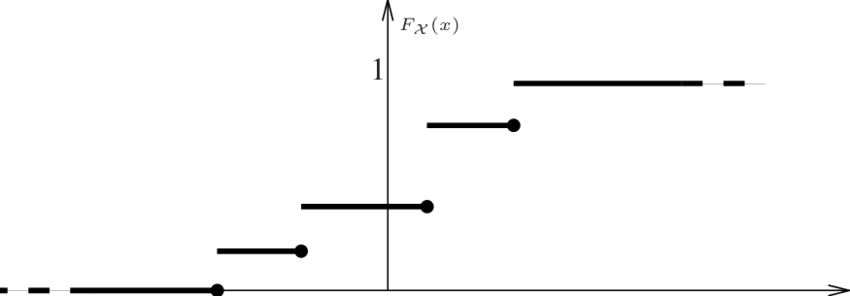
\includegraphics[scale=0.3]{figures/fct-rep-disc.png}
    \caption{Exemple de fonction de répartition d'une variable aléatoire discrète.}
    \label{}
  \end{figure}

  \begin{remark}[Notations]
    Mesure de Lebesgue :   $\begin{cases}
      \text{Leb} \\
      dx
    \end{cases}$
  \end{remark}

  \item Soit $\nu$ une mesure de probabilité de Borel sur $\mathbb{R}$. On dira que $\nu$ est \textbf{absolument continue} s'il existe une fonction non-négative $f \in L ^{1}(\text{Leb}) \ (\int_{\mathbb{R}}^{} f dx \less \infty )$ telle que, pour tout borelien $B$,

  \begin{equation*}
    \nu(B) = \int_{B}^{} f(x) dx.
  \end{equation*}

  \emph{On la dénote aussi $\nu \ll \text{Leb}$.}

  En particulier si $g$ est bornée ($L ^{\infty}(\text{Leb})$), alors

  \begin{equation*}
    \int_{\mathbb{R}}^{} g d \nu = \int_{\mathbb{R}}^{} gf dx.
  \end{equation*}

  $f$ est la densité de $f$ par rapport à Lebesgue (dérivée de Radon-Nykodym).

\end{enumerate}

Dans notre cas, $\nu((a,b]) = F(b)-F(a)$.

Si $F$ est la fonction de répartition de $X$, on a

\begin{gather*}
  P_X((a,b]) = F(b)-F(a) \stackrel{\text{Si la loi est AC}}{=} \int_{(a,b]}^{} f(x)dx \\
   = \int_{[a,b]}^{} f(x) dx = \underbrace{\int_{a}^{b} f(x) dx }_{\text{Intégrale de Riemann}}
\end{gather*}

\begin{definition}[Variable aléatoire à densité]
  On dira qu'une variable aléatoire $X$ est \textbf{à densité} si sa loi est absolument continue et on appelle $f_X$ la densité de probabilité de $X$.
\end{definition}

Si $\nu = c_1 \delta _{X_1} + c_2 \text{Leb}$, on écrit $\nu(A) = c_1 \delta _{X_1}(A) + c_2 \text{Leb} (A)$.

Il n'y a pas de saut dans la fonction de répartition d'une variable aléatoire absolument continue, car si $F(b) - F(a) = \int_{a}^{b} f(t) dt $, on a $$\text{saut}(x_0) = F(x_0) - F(x_0 ^{-}) = 0.$$

C'est lié au fait que pour $\lambda$ mesure de Lebesgue, on a $\lambda (\{ b \} ) = 0$ (cf \ref{lebesgue-zero}).

\begin{thm}
  Toute fonction de répartition $F$ s'écrira (pour nous) de la forme

  \begin{equation*}
    F(t) = c_1 F _{\text{d} }(t) + c_2 F _{\text{ac}}(t),
  \end{equation*}

  où $F _{\text{d}}$ est la fonction de répartition d'une variable aléatoire discrète et $F _{\text{ac}}$ est la fonction de répartition d'une variable aléatoire absolument continue et $c_1+c_2 = 1$.
\end{thm}

Dans ce cas, $P_X = c_1 (\text{masses de Dirac}) + c_2(\text{mesure absolument continue})$.

\

Soit $X$ une variable à densité $f_X$. Soit $g :  \mathbb{R} \to \mathbb{R}$. On considère la même variable aléatoire $g \circ X$. Quelle est sa loi ?


\begin{exemple}
  Soit une variable aléatoire $X$ avec la loi exponentielle. $X : \Omega \longrightarrow \mathbb{R}$,

  \begin{gather*}
    f_X(x) = e^{-x} \mathds{1} _{[0, \infty)}(x).
  \end{gather*}

  Trouver la loi de $X ^2 = g \circ X$, avec $g : x \to x ^2$.
\end{exemple}

Soit $h$ une fonction bornée positive quelconque (fonction test).

\begin{gather}
  \int _{\Omega} h(g(X)) d \mathbb{P} = \int _{\Omega} (h \circ g) (X) d \mathbb{P} \stackrel{\text{transfert}}{=} \int_{\mathbb{R}} (h \circ g)(x) d P_X(x) \\
  = \int_{\mathbb{R}}^{} (h \circ g)(x) f_X(x) dx = \int_{A}^{} h(g(x)) f_X(x) dx. \label{chgt-var}
\end{gather}

On fait un changement de variable en posant $y=g(x), d y = g'(x) dx$.

Dans ce cas, \ref{chgt-var} devient

\begin{gather*}
\int h(y) f_X (g ^{-1} (y)) dy.
\end{gather*}

Or

\begin{gather*}
  \int h(y) c(y) dy = \int_{g(A)}^{} h(y)  f_X(g ^{-1} (y)) \frac{1}{g' (g ^{-1} (y))}dy,
\end{gather*}

avec $c$ la densité associée à $y = g(x)$ et $(g ^{-1} )' = \displaystyle\frac{1}{g'(g ^{-1})}$.


Comme $h$ est quelconque,

\begin{gather*}
  c(y) = f_X(g ^{-1}(y) ) \frac{1}{g' (g ^{-1} (y))} \mathds{1} _{g(A)} (y).
\end{gather*}

Dans notre exemple, $X$ a la densité $f_X(x) = e^{-x} \mathds{1} _{[0, \infty)}(x) $ et $g(x) = x ^2$, $A = [0, \infty)$.

On a

\[
\begin{matrix}
  y = x ^2 \\
  x= \sqrt{ y }.
\end{matrix}
\]


On obtient

\begin{gather*}
  \overbrace{c(y)}^{\text{densité} X ^2 } = e^{- \sqrt{ y } } \mathds{1} _{[0, \infty)}(y) \frac{1}{2 \sqrt{ y } } \mathds{1} _{g([0, \infty))}(y) \\
  = \frac{e^{-\sqrt{ y } } }{2 \sqrt{ y } } \mathds{1} _{[0, \infty)} (y),
\end{gather*}

car $g([0, \infty)) = [0, \infty)$.

\begin{exemple}
  $X$ suit la loi uniforme entre $[-1, 1]$.

  $f_X = \frac{1}{2}\mathds{1}_{[-1, 1]} $, car $\displaystyle \frac{1}{2} \int_{-1}^{1}dt = 1 $.  Calculer $X ^2$.
\end{exemple}

\begin{gather*}
  \int_{}^{} h(g(X)) d \mathbb{P} = \int_{}^{} (h \circ g) (X) d \mathbb{P} = \int_{-1}^{1} (h \circ g)(x) f_X(x) dx \\
  = \int_{-1}^{0} (h \circ g)(x) f_X(x) dx + \int_{0}^{1} (h \circ g)(x) f_X(x) dx \\
  = \int_{0}^{1}  h(y) f_X(- \sqrt{ y } ) \frac{1}{2 \sqrt{ y } } dy + \int_{0}^{1} h(y) f _{X} (\sqrt{ y } ) \frac{1}{2 \sqrt{ y } } dy \\
  = \int_{0}^{1} h(y) \frac{1}{2 \sqrt{ y } } [f_X(-\sqrt{ y } ) + f_X(\sqrt{ y } )] dy.
\end{gather*}

On a

\begin{equation*}
  \int h (g(X)) d \mathbb{P} = \int h(y) c_Y(y) dy,
\end{equation*}

avec

\begin{equation*}
  c_Y(y) = \frac{1}{2 \sqrt{ y } } [f_X(- \sqrt{ y } )+ f_X(\sqrt{ y } )] \mathds{1}_{[0, 1]}(y).
\end{equation*}

\

Soit $(\Omega, \mathscr{A}, \mathbb{P} )$ un espace probabilisé. Soit $B \in \mathscr{A}, \mathbb{P}(B) \bg 0 $.

On peut définir $\mathbb{P}(A \mid B)$, la probabilité conditionnelle de $A$ sachant $B$, définie comme suit :

\begin{equation*}
  \mathbb{P}(A \mid B) = \frac{\mathbb{P}(A \cap B)}{ \mathbb{P}(B)}.
\end{equation*}

\begin{exo}
  Si l'on fixe $B$, montrer que $\mathbb{P}(\cdot \mid B) \to [0, 1]$ est une probabilité.
\end{exo}

On dira que deux événements $A$ et $B$ sont \textbf{indépendants} si $\mathbb{P}(A \cap B) = \mathbb{P}(A) \iff \mathbb{P}(A \cap B) = \mathbb{P}(A) \mathbb{P}(B)$, avec $\mathbb{P}(B) \bg 0$.

\section{Système complet d'événements}


\begin{definition}
  Soit
  \[
  \Omega = \bigcup_{i=1} ^{\infty} A_i,
  \]

  avec $A_i \cap A_j = \emptyset$ si $i \neq j$ et $\forall i \geq  1, \mathbb{P}(A_i) \bg 0$.



  On appelle $ \displaystyle \{ A_i \} _{i=1} ^{\infty}$ un \textbf{système complet d'événements} (SCE).
\end{definition}

\begin{thm}[Formule des probabilités totales]
  Si $B \in \mathscr{A} $ quelconque, alors

  \begin{gather*}
    \mathbb{P}(B) = \sum_{i=1}^{\infty} \mathbb{P}(B \cap A_i) = \sum_{i=1}^{\infty} \mathbb{P}(B \mid A_i) \mathbb{P}(A_i).
  \end{gather*}
\end{thm}

\marginnote{22-09-2023}

\chapter{Vecteurs aléatoires}

On considère maintenant des variables aléatoires $X : (\Omega, \mathscr{A}, \mathbb{P} ) \longrightarrow \mathbb{R}^n$ (\bsc{Borel} engendrée par les ouverts).

On étudiera surtout les cas où $n=2$. On dénote un vecteur aléatoire $X \equiv (X_1, X_2)$ (parfois $(X, Y)$). Parfois on écrit, pour $i = 1, \dots, n$,

\[
X_i = \pi_i \circ X, \text{ où } \pi_i :  \mathbb{R}^n \to \mathbb{R}, \pi_i(x_1, \dots, x_n) = x_i.
\]

$\pi_i$ est une \textbf{projection}.

\begin{definition}[Loi d'un vecteur aléatoire]
  Soit $B$ un borélien de $\mathbb{R}^n$. Alors la loi de $X$ (loi conjointe) est définie ainsi :

  \[
  P_X (B) = \mathbb{P}(\omega \in \Omega, X(w) = (X_1(\omega), \dots, X_n(\omega)) \in B) = \mathbb{P}(X ^{-1} (B)).
  \]
\end{definition}

\emph{Est-il possible de calculer la loi de $X_1$?}

Si on connaît la loi du couple de variables aléatoires, il est possible de calculer les lois des deux variables. Par contre, on ne peut pas avoir la loi du couple en connaissant la loi des deux variables aléatoires.

\begin{definition}[Loi marginale]
  Si $D$ est un borélien de $\mathbb{R}$, la loi de $X$ est

  \begin{gather*}
    \underbrace{P _{X_1}(D)}_{\text{loi marginale}} = \mathbb{P}(X_1 \in D) = \mathbb{P}(\pi_1 \circ X \in D) = \mathbb{P}(X \in \pi_1 ^{-1} (D)) = P_X(\underbrace{\pi_1 ^{-1} (D)}_{\text{borélien}}).
  \end{gather*}
\end{definition}

\begin{remark}
  $\pi_i ^{-1} (D)$ est borélien, car $\pi_i$ est continue.
\end{remark}


\section{Fonction de répartition}

Dans le cas où $n=2$, $X = (X_1, X_2)$,

\begin{gather*}
  F_X(t_1, t_2) = \mathbb{P}(X_1 \leq t_1, X_2 \leq t_2) = P_X((-\infty, t_1] \times (-\infty, t_2]).
\end{gather*}


\begin{definition}
  On dira que le vecteur aléatoire $X$ est \textbf{absolument continu} s'il existe une fonction $f$ mesurable et \textbf{non-négative} définie comme $f : \mathbb{R}^2 \to \mathbb{R}$ telle que, pour tout borélien $B$ de $\mathbb{R}^2$, on a

  \[
  P _{X}(B) = P _{(X_1, X_2)}(B) = \iint_{B} \underbrace{f(x_1, x_2)}_{\text{densité du couple}} dx_1 dx_2
  \]

  et si $B = (-\infty, t_1] \times (-\infty, t_2]$, alors

  \begin{gather*}
    F_X(t_1, t_2) = \int_{-\infty}^{t_1} \int_{-\infty}^{t_2} f(x_1, x_2) dx_1dx_2 = \iint_{\mathbb{R}^2} f(x_1, x_2) \mathds{1}_{(-\infty, t_1]}(x_1) \mathds{1}_{(-\infty, t_2]}(x_2) dx_1 dx_2.
  \end{gather*}
\end{definition}

\begin{prop}

  \

  \begin{gather*}
    F _{X_1} (t_1) = \lim_{t_2 \to \infty} F _{(X_1, X_2)} (t_1, t_2)  \text{ et } F _{X_2} = \lim_{t_1 \to \infty} F _{(X_1, X_2)} (t_1, t_2).
  \end{gather*}
\end{prop}

\begin{proof}
  \begin{gather*}
    F _{X_1}(t_1) = \mathbb{P}(X_1 \leq t_1) = \mathbb{P}(X_1 \leq t_1, \underbrace{X_2 \in \mathbb{R}}_{\text{toujours vrai}}),
  \end{gather*}

  car

  \begin{gather*}
    \{  X_1 \leq t_1 \} = \{ \omega, X_1(\omega) \leq t_1 \} = \{ \omega, X_1(\omega) \leq t_1 \} \cap \Omega = \{ \omega, X_1 (\omega)\leq t_1 \} \cap \underbrace{X_2 ^{-1} (\mathbb{R})}_{X_2 \in \mathbb{R}}).
  \end{gather*}

  Donc

  \begin{gather*}
    F _{X_1}(t) = \mathbb{P}(X_1 \leq t_1, X_2 \in \mathbb{R}) = P _{X_1, X_2} ((- \infty, t_1] \times \mathbb{R}) = \lim_{k \to \infty} P _{X_1, X_2} ((-\infty, t_1] \times (-\infty, k]),
  \end{gather*}

  car
  \[
  \left((-\infty, t_1] \times \bigcup _{k=1} ^{\infty} (-\infty, k)\right) = (-\infty, t_1] \times \mathbb{R}.
  \]

  Ainsi

  \begin{gather*}
    \lim_{k \to \infty} P _{X_1, X_2} ((-\infty, t_1] \times (-\infty, k]) = \lim_{k \to \infty} F _{(X_1, X_2)} (t_1, k), k \in \mathbb{R}.
  \end{gather*}
\end{proof}

\begin{thm}[De transfert pour un vecteur aléatoire]
  Soit $g$ une fonction mesurable. Alors on a
  \begin{gather*}
    \int_{\Omega}^{} g(X) d \mathbb{P} = \int_{\Omega}^{} g((X_1, X_2)) d \mathbb{P} = \iint_{\mathbb{R}^2} g(x_1, x_2) d P_X(x_1, x_2) = \iint_{\mathbb{R}^2}   g(x_1, x_2) f_X(x_1, x_2) dx_1dx_2.
  \end{gather*}
\end{thm}

\begin{prop}
  Soit $X = (X_1, X_2)$ absolument continu, donc il existe une densité $f_X(x_1, x_2)$. Alors on a

  \[
  \begin{cases}
    f _{X_1}(x_1) = \int_{\mathbb{R}} f _{(X_1, X_2)} (x_1, x_2) d x_2, \\
    f _{X_2}(x_2) = \int_{\mathbb{R}} f _{(X_1, X_2)} (x_1, x_2) d x_1.
  \end{cases}
  \]
\end{prop}

\begin{proof}
  Si $X_1$ a une densité, cela signifie

  \[
  F _{X_1} (t_1) = \int_{-\infty}^{t_1} f _{X_1} (x_1) dx_1.
  \]

  \emph{Ce résultat est-il vrai ?}

  Par le théorème précédent,

  \begin{gather*}
    F _{X_1}(t_1) = \lim_{t_2 \to \infty} F _{(X_1, X_2)} (t_1, t_2) = \lim_{t_2 \to \infty} \int_{-\infty}^{t_1} \int_{-\infty}^{t_2} f _{(X_1, X_2)} (u_1, u_2) d u_1 u_2 \\
    = \lim_{t_2 \to \infty} \iint_{ \mathbb{R}^2} f _{(X_1, X_2)} (u_1, u_2) \mathds{1}_{(-\infty, t_1]}(u_1) \mathds{1}_{(-\infty, t_2]}(u_2) d u_1 d u_2   \\
    = \lim_{t_2 \to \infty} \int_{\mathbb{R}}^{}\mathds{1}_{(-\infty, t_1]}(u_1) \left[ \int_{\mathbb{R}}^{} f _{(X_1, X_2)}(u_1, u_2) \mathds{1}_{(-\infty , t_2]}(u_2) d u_2 \right]d u_1 \\
    = \int_{\mathbb{R}} \mathds{1}_{(-\infty, t_1]}(u_1) \int_{\mathbb{R}} f _{(X_1, X_2)} (u_1, u_2) d u_2 d u_1  = \int_{-\infty}^{t_1} \left(\int_{\mathbb{R}} f _{(X_1, X_2)} (u_1, u_2) d u_2 \right) d u_1.
  \end{gather*}
\end{proof}

\chapter{Indépendance}

Soit $(\Omega, \mathscr{A}, \mathbb{P} )$ un espace probabilisé.

\section{Evénements indépendants}


\begin{definition}
  Deux événements $A, B \in \mathscr{A}$ sont indépendants si

  \[
  \mathbb{P}(A \cap B) = \mathbb{P}(A) \mathbb{P}(B)
  \]

  ou

  \[
  \mathbb{P}(A \mid B) = \mathbb{P}(A) \text{ si } \mathbb{P}(B) \bg 0.
  \]
\end{definition}

\section{Mutuellement indépendants}

\begin{definition}
  Soit $\{ A_n \} $ une suite dénombrable d'événements. On dira que cette suite est \textbf{mutuellement indépendante} si pour toute sous-suite d'événements $A _{i_1}, \dots, A _{i_k}$, on a

  \[
  \mathbb{P}(A _{i_1} \cap A _{i_2} \cap \dots \cap A _{i_k}) = \mathbb{P}(A _{i_1}) \mathbb{P}(A _{i_2}) \dots \mathbb{P}(A _{i_k}).
  \]
\end{definition}

\section{Classes d'événements indépendantes}

\begin{definition}
  Deux classes d'événements $\mathscr{C}_1 $ et $\mathscr{C}_2 $ sont dites indépendantes si $\forall A_1 \in \mathscr{C}_1 $ et $A_2 \in \mathscr{C}_2 $, $A_1$ et $A_2$ sont indépendants.

  Cela se généralise à $n$ classes $\mathscr{C}_1, \dots, \mathscr{C}_n$.
\end{definition}

\begin{definition}\label{sigma-alg-indep}
  Soit $\mathscr{C}_1 $ et $\mathscr{C}_2 $ deux classes d'événements indépendants et en plus qui sont \textbf{stables par intersection finie} ($\pi$-système). Alors les $\sigma$-algèbres engendrées par $\mathscr{C}_1 $ et $\mathscr{C}_2 $ sont indépendantes.
\end{definition}

\begin{definition}
  Soit $\mathscr{C} $ une classe. Soient $C_1, C_2, \dots, C_n \in \mathscr{C} $. On dira que $\mathscr{C} $ est stable par intersection finie si

  \[
  C_1 \cap C_2 \cap \dots \cap C_n \in \mathscr{C}.
  \]
\end{definition}

\begin{exemple}
  \begin{enumerate}
    \item Dans $\mathbb{R}$, on considère la classe $\mathscr{C}_1 = \{ (a,b], a, b \in \mathbb{R} \} $. C'est un $\pi$-système, car pour tout $(a,b], (c,d]$, on aura

    \[
    (a,b] \cap (c,d] = (\max \{ a,c \}, \min \{ b,d \} ].
    \]
  \end{enumerate}
\end{exemple}


%Prenons dans $\mathbb{R}$ la classe $\mathscr{C}_1  = \{ (a,b] \} $. C'est un $\pi$-système.

Dans $\mathbb{R}^2$, $\mathscr{C} = \{ (a_1,b_1] \times (a_2, b_2] \} $. Alors $\sigma(\mathscr{C} ) = \sigma$-algèbre de \bsc{Borel} dans $\mathbb{R}^2$.

\begin{definition}
  Soit $X :  \Omega \longrightarrow \mathbb{R}$ une variable aléatoire telle que $X ^{-1} (\beta ) \subset \Omega$. On appelle $\sigma(X)$ la plus petite $\sigma$-algèbre qui rend $X$ mesurable.
\end{definition}

\begin{prop}
  \[
  \sigma(X) = X ^{-1} (\beta ),
  \]

  où $\beta $ est la $\sigma$-algèbre de \bsc{Borel} dans $\mathbb{R}$.
\end{prop}

\begin{remark}[Personnelle]
  Soient $E_1, E_2$ ensembles et $f : E_1 \to E_2$. On rappelle que si $\tau_2$ est une tribu sur $E_2$, alors

  \[
  f ^{-1} (\tau_2) = \{ f ^{-1} (A), A \in \tau_2 \}
  \]

  est une tribu sur $E_1$, appelée \textbf{la tribu réciproque}.

  Dans le cas de probabilités, on aura

  \[
  X ^{-1} (\beta ) = \{ X ^{-1} (B), B \text{ borélien}  \}.
  \]
\end{remark}

%Etudions le cas de figure où la fonction est définie comme suit :

\begin{figure}[h!]
  \centering
  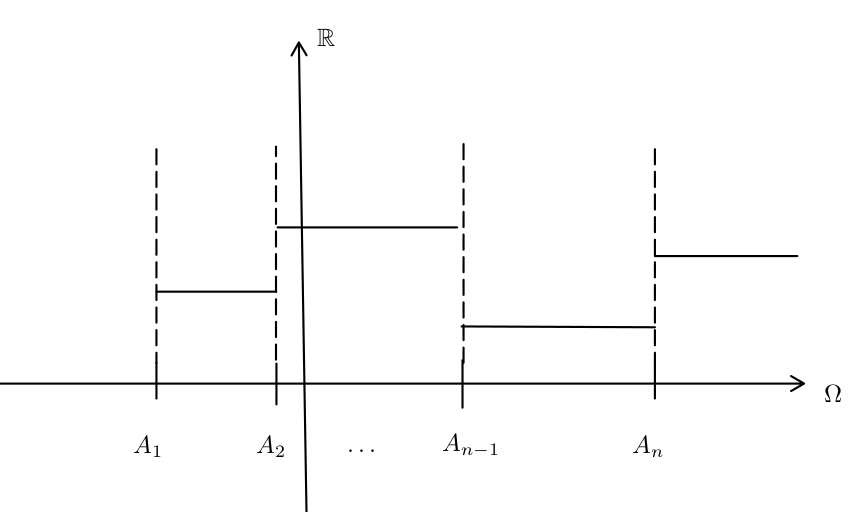
\includegraphics[scale=0.3]{figures/sigma_n.png}
  \caption{Dans ce cas, $\sigma(X) = \sigma$-algèbre engendrée par la partition $\mathscr{A}$.}
  \label{ss-x-partition}
\end{figure}

\begin{remark}[Personnelle]
  On rappelle que pour la figure \ref{ss-x-partition}, si \(A_1, \dots, A_n\) est une partition de l'ensemble \(X\), on définit

  \[
  \tau = \left\{ \bigcup _{i \in J} A_i, J \subset \{ 1, \dots, n \} \right\}.
  \]

  On démontre que $\tau$ est une tribu.
\end{remark}

\section{Indépendance de variables aléatoires}


\begin{definition}
  Deux variables aléatoires $X_1, X_2$ sont indépendantes si $\sigma(X_1) = X_1 ^{-1} (\beta )$ et $\sigma(X_2) = X_2 ^{-1} (\beta )$ sont deux \textbf{familles indépendantes} (cf définition \ref{sigma-alg-indep}).
\end{definition}

Un élément de $X ^{-1} (\beta )$ s'écrit comme $X ^{-1} (B_1), B_1 \in \beta$.

On écrira alors

\[
\mathbb{P}(X_1 ^{-1} (B_1) \cap X_2 ^{-1} (B_2)) = \mathbb{P}(X_1 ^{-1} (B_1)) \mathbb{P}(X_2 ^{-1} (B_2)).
\]

On aura par conséquent, pour $(-\infty, b]$ qui engendrent $\beta$ (\( \{ (-\infty, b] \} \) est un \(\pi\)-système),

\[\mathbb{P}(X_1 ^{-1} ((-\infty,b_1]) \cap X_2 ^{-1} (-\infty,b_2]) = \mathbb{P}(X_1 ^{-1} (-\infty,b_1]) \mathbb{P}(X_2 ^{-1} (-\infty, b_2]), \]

donc

\[\mathbb{P}(X_1 \in (-\infty, b_1], X_2 \in (-\infty, b_2]) = \mathbb{P}(X_1 \in (-\infty,b_1]) \mathbb{P}(X_2 \in (-\infty, b_2]).\]

On obtient ainsi

\begin{equation}
  \mathbb{P}(X_1 \leq b_1, X_2 \leq b_2)  = \mathbb{P}(X_1 \leq b_1) \mathbb{P}(X_2 \leq b_2). \label{indep-def}
\end{equation}


\marginnote{25-09-2023}

Le résultat \ref{indep-def} est exactement la définition de l'indépendance des deux variables aléatoires.

On peut écrire \ref{indep-def} en terme de lois de probabilités :


\begin{equation}\label{indep-loi}
  \mathbb{P}(\overbrace{X_1 \leq b_1, X_2 \leq b_2}^{\subset \Omega}) = P_X((-\infty, b_1] \times (-\infty, b_2]) \stackrel{\text{si indép}}{=} P _{X_1}((-\infty, b_1]) P _{X_2}((-\infty, b_2]).
\end{equation}


\begin{prop}
  Deux variables aléatoires \(X_1, X_2\) définies sur l'espace \((\Omega, \mathscr{A}, \mathbb{P} )\) sont indépendantes si et seulement si

  \[P _{(X_1, X_2)} = P _{X_1} P _{X_2}.\]
\end{prop}

\begin{proof}

  \

  \begin{enumerate}
    \item \emph{Partie nécessaire.} On l'a démontré dans \ref{indep-loi}.
    \item \emph{Partie suffisante.} On suppose que

    \[\overbrace{P _{(X_1, X_2)}(B_1 \times B_2)}^{\text{loi du couple}}  = P _{X_1}(B_1) P _{X_2}(X_2).\]

    On prend $B_1 =(-\infty, b_1]$ et \(B_2 = (-\infty, b_2]\).

    Ainsi

    \[P _{(X_1, X_2)}((-\infty, b_1] \times (-\infty,b_2]) = \mathbb{P}(X_1 \leq b_1, X_2 \leq b_2).\]
  \end{enumerate}
\end{proof}


\begin{exemple}
  Considérons un vecteur aléatoire \((X_1, X_2)\) de loi

  \[\begin{cases}
     P _{X_1} = \frac{1}{2} \delta _{a_1} + \frac{1}{2}\delta _{a_2} = f_1(y)dy \\
     P _{X_2} = f_2(x) dx.
  \end{cases}\]

  On veut trouver la loi de \((X_1, X_2)\).
\end{exemple}

On calcule :

\begin{gather*}
  \int_{}^{} e^{X_1+X_2} d \mathbb{P} = \iint_{} e^{x_1+x_2} d P _{(X_1, X_2)} P(x_1, x_2) = \iint e^{x_1+x_2} d\left(\frac{1}{2} \delta _{a_1} + \frac{1}{2}\delta _{a_2}\right)f_2 d x_2 = \dots
\end{gather*}

\begin{corollary}
  Si $X_1, X_2$ sont indépendantes, la même chose est vraie pour $f(X_1)$ et $g(X_2)$ avec $f$ et $g$ réelles et mesurables.
\end{corollary}

\begin{prop}
  Les variables aléatoires $X_1$ et $X_2$ sont indépendantes si et seulement si pour toutes $f, g$ non-négatives, on a

  \[\mathbb{E}[ f(X_1)g(X_2) ] = \mathbb{E}[ f(X_1) ] \mathbb{E}[ g(X_2) ]\]

  et la même chose pour $f$ et $g$ réelles et bornées.
\end{prop}

\begin{proof}

  \begin{enumerate}
    \item \emph{Partie nécessaire.}

    \begin{equation}
      \int_{\Omega}^{} f(X_1)g(X_2) d \mathbb{P} = \iint_{\mathbb{R}^2} f(x_1) g(x_2) d _{X_1 X_2} P(x_1, x_2).  \label{marg}
    \end{equation}

    Or si les variables sont indépendantes, la loi \(P _{X_1 X_2}\) se factorise dans les marginales.

    Donc \ref{marg} devient :

    \begin{gather*}
      \iint_{\mathbb{R}^2} f(x_1)g(x_2) d P_{X_1}(x_1) d P _{X_2}(x_2) = \int_{\mathbb{R}}^{} f(x_1) d P _{X_1}(x_1) \int_{\mathbb{R}}^{} g(x_2) d P _{X_2}(x_2) = \mathbb{E}[X_1] \mathbb{E}[X_2].
    \end{gather*}

    \item \emph{Partie suffisante.} On considère $f = \mathds{1}_{(-\infty, b_1]} \text{ et } g= \mathds{1}_{(-\infty,b_2]}. $

    On a

    \begin{gather*}
      \int_{}^{} \mathds{1}_{(-\infty, b_1]} \circ X_1 \mathds{1}_{(-\infty, b_2]} \circ X_2 d \mathbb{P} = \mathbb{E}[f(X_1)g(X_2)] = \mathbb{E}[f(X_1)] \mathbb{E}[g(X_2)] = \mathbb{P}(X_1 \leq b_1) \mathbb{P}(X_2 \leq b_2).
    \end{gather*}


  \end{enumerate}

\end{proof}

  \begin{prop}[Indépendance et fonctions de répartition]
    Les variables aléatoires $X_1$ et $X_2$ sont indépendantes si et seulement si

    \[F _{X_1, X_2}(t_1, t_2) = F _{X_1}(t_1) F _{X_2}(t_2).\]
  \end{prop}

  \begin{proof}
    \begin{enumerate}
      \item \emph{Partie nécessaire.} Si les variables aléatoires \(X_1, X_2\) sont indépendantes, alors

      \begin{gather*}
        F _{X_1, X_2}(t_1, t_2) = \mathbb{P}(X_1 \leq t_1, X_2 \leq t_2) = \mathbb{P}(X_1 \leq t_1) \mathbb{P}(X_2 \leq t_1) = F _{X_1}(t_1) F _{X_2}(t_2).
      \end{gather*}

      \item \emph{Partie suffisante.} Point de départ : on écrit la condition

      \[  \mathbb{P}(X_1 \leq t_1, X_2 \leq t_2) = F _{X_1 X_2}(t_1, t_2) = F _{X_1}(t_1) F _{X_2}(t_2)= \mathbb{P}(X_1 \leq t_1) \mathbb{P}(X_2 \leq t_2) ,\]

      avec \(t_1, t_2\) quelconques et on obtient que \(X_1 \text{ et } X_2 \) sont indépendantes comme c'est dit dans la définition \ref{indep-def}.
    \end{enumerate}
  \end{proof}

  \begin{prop}[Indépendance et densités]

    \

    \begin{enumerate}
      \item Soient $X_1, X_2$ deux variables aléatoires avec les densités $f _{X_1}$ et $f _{X_2}$ et supposons que \(X_1\) et \(X_2\) sont indépendantes. Alors le couple \((X_1, X_2)\) et sa densité vérifient :

      \[f _{X_1, X_2}(x_1, x_2) = f _{X_1}(x_1) f _{X_2}(x_2).\]

      \item Supposons que $(X_1, X_2)$ admet la densité $f _{X_1, X_2}(x_1, x_2)$ qui est le produit entre deux fonctions intégrables non-négatives $\tilde{f}_1(x_1), \tilde{f}_2(x_2)$. Alors $\tilde{f}_1(x_1)$ et \(\tilde{f}_2(x_2)\) sont à des facteurs multiplicatifs près, les densités de \(X_1\) et \(X_2\) sont \textbf{indépendantes}.
    \end{enumerate}

\end{prop}

%ъуъ

\begin{proof}

  \

  \begin{enumerate}
    \item Loi de \(X_1 \implies f _{X_1}(x_1) d x_1 : P _{X_1}\) et loi de \(X_2 \implies f _{X_2} (x_2) d x_2 : P _{X_2}\).

    \[f _{X_1, X_2}(x_1, x_2)dx_1dx_2 = P _{X_1 X_2} = P _{X_1} P _{X_2} = f _{X_1}(x_1) f _{X_2}(x_2) dx_1dx_2.\]

    \item On sait que

    \begin{gather*}
      f _{X_1}(x_1) = \int_{}^{} f _{X_1 X_2}(x_1, x_2) d x_2 = \tilde{f} _{X_1}(x_1) \int_{}^{} \tilde{f} _{X_2} (x_2) d x_2  \\
      f _{X_2}(x_2) = \int_{}^{} f _{X_1 X_2} (x_1, x_2) d x_1 = \tilde{f} _{X_2}(x_2) \int_{}^{} \tilde{f} _{X_1}(x_1) d x_1.
    \end{gather*}

    Ensuite,

    \begin{gather*}
      \iint_{\mathbb{R}^2} f _{X_1 X_2}(x_1, x_2) dx_1dx_2 = 1 = \iint_{\mathbb{R}^2} \tilde{f} _{X_1}(x_1) \tilde{f} _{X_2}(x_2) dx_1dx_2 = \int_{\mathbb{R}}^{} \tilde{f}(x_1) dx_1 \int_{\mathbb{R}}^{} \tilde{f}_{X_2}(x_2) dx_2.
    \end{gather*}

    On a

    \begin{gather*}
      f _{X_1}(x_1) f _{X_2}(x_2) = \tilde{f}_{X_1}(x_1) \tilde{f} _{X_2}(x_2) \underbrace{\int_{}^{} \tilde{f} _{X_2}(x_2) d x_2 \int_{}^{} \tilde{f}_{X_1} (x_1) d x_1}_{=1}.
    \end{gather*}

    En conclusion, on a

    \[ f _{X_1}(x_1) f _{X_2}(x_2) = \tilde{f} _{X_1}(x_1) \tilde{f} _{X_2}(x_2).\]

    Pour que $f _{X_1}$ et $f _{X_2}$ deviennent des densités, on pose :

    \[f _{X_1}(x_1) = \frac{\tilde{f} _{X_1}(x_1)}{\int_{}^{}f _{X_1}(x_1) d x_1 } \text{ et } f _{X_2}(x_2) = \frac{\tilde{f} _{X_2}(x_2)}{\int_{}^{}f _{X_2}(x_2) d x_2 }. \]
  \end{enumerate}
\end{proof}

%Réviser changement de variable dans \mathbb{R}^n.



\marginnote{26-09-2023}

%Programme :
%Convergence de VA
%Convergence en loi (fonction caractéristique)
%Théorèmes limites
%Vecteurs gaussiens
%(Espérances conditionnelles)

\section{Changement de variables}

On considère \((X_1, X_2)\) un vecteur aléatoire à densité \(f _{X_1 X_2}(x_1, x_2)\). On construit deux autres variables aléatoires \(U_1, U_2\) telles que

\[\begin{cases}
U_1 = g_1(X_1, X_2) \\
U_2 = g_2(X_1, X_2).
\end{cases}\]


On veut trouver la loi de \(U_1, U_2\), à savoir la densité du couple.

Soit \(h : \mathbb{R}^2 \to \mathbb{R}\) une fonction mesurable positive quelconque que l'on appelle ``fonction test''.

\begin{gather}
  \int_{\Omega} h(U_1, U_2) d \mathbb{P} = \int_{\Omega} h(g_1(X_1, X_2), g_2(X_1, X_2)) d \mathbb{P} \\
  \stackrel{\text{transfert}}{=} \iint_{\mathbb{R}^2} h (g_1(x_1, x_2), g_2(x_1, x_2)) d P _{X_1 X_2}\\
  = \iint_{\mathbb{R}^2} h(g_1(x_1, x_2), g_2(x_1, x_2)) f _{X_1, X_2} (x_1, x_2) d x_1 d x_2. \label{chva}
\end{gather}

On pose

\[\begin{cases}
u_1 = g_1 (x_1, x_2) \\
u_2 = g_2 (x_1, x_2).
\end{cases}\]

On sait que \((X_1, X_2)\) ne sont pas forcément définies sur \(\mathbb{R}^2\), mais sur un certain domaine \(A \subset \mathbb{R}^2\). On pose \(G = (g_1, g_2) : \mathbb{R}^2 \to \mathbb{R}^2\).

On doit avoir \(G ^{-1}  : \begin{cases}
  x_1 = d_1(u_1, u_2) \\
  x_2 = d_2(u_1, u_2)
\end{cases},\) donc il faut que \(G\) soit inversible. De plus, on devrait calculer la matrice jacobienne

\[J _{U_1 U_2} = \left(\begin{matrix}
  \frac{\partial d_1 }{\partial u_1 } & \frac{\partial d_1 }{\partial u_2} \\
  \frac{\partial d_2 }{\partial u_2 } & \frac{\partial d_2 }{\partial u_2}
\end{matrix}\right).\]

\ref{chva} devient :

\begin{gather*}
  \iint_{\mathbb{R}^2 \cap G(A)} h(u_1, u_2) f _{X_1 X_2} (d_1(u_1, u_2), d_2(u_1, u_2)) \lvert \operatorname{det}(J _{U_1 U_2}(u_1, u_2)) \rvert d u_1 d u_2.
\end{gather*}

Comme \(h\) est quelconque, on peut choisir \(h(x) = \mathds{1}_{\{ g \bg f \} }(x) \text{ et puis } h(x) = \mathds{1}_{\{ g \less f \} } \).

On obtient la formule de changement de variable :

\begin{thm}[Formule de changement de variables]
  \[f _{U_1 U_2}(u_1, u_2) = f _{X_1 X_2}(d_1(u_1, u_2), d_2(u_1, u_2)) \lvert \operatorname{det} J _{U_1 U_2}(u_1, u_2) \rvert \mathds{1}_{G(A)}(u_1, u_2).\]
\end{thm}

\emph{Si on a deux variables aléatoires \(X_1 \text{ et } X_2 \), quelle est la loi de \((X_1+X_2)\) ?}

On introduit \[\begin{cases}
  U_1 = X_1 + X_2,
  U_2 = X_2
\end{cases} \implies \begin{cases}
  X_1 = U_1 - U_2 \\
  X_2 = U_2
\end{cases}.\]

De plus, \[J _{U_1 U_2} = \begin{pmatrix}
1 & -1 \\
0 & 1
\end{pmatrix}.\]

On calcule \[f _{U_1 U_2} (u_1, u_2) = f _{X_1 X_2}(u_1 - u_2, u_2)\] et on obtient \[f _{U_1}(u_1) = \int f _{U_1, U_2}(u_1, u_2) d u_2 = \int_{}^{} f _{X_1 X_2} (u_1 - u_2, u_2) d u_2 = \int_{\mathbb{R}}^{} f _{X_1}(u_1- u_2)f _{X_2}(u_2) d u_2. \]

Il s'agit du \textbf{produit de convolution}.

\chapter{Convergence des variables aléatoires} \marginnote{02-10-2023}

On a une suite de variables aléatoires \(\{ X_n \} _{n=1} ^{\infty} \) toutes définies sur \((\Omega, \mathscr{A}, \mathbb{P})\).

Comment calculer \(\lim_{n \to \infty} X_n\) ?

\begin{enumerate}
  \item Convergence ``en probabilité'';
  \item Convergence ``en moyenne'';
  \item Convergence ``presque sûre'' ;
  \item Convergence ``en loi'' \(\longrightarrow\) Théorème central limite.
\end{enumerate}


\section{Convergence en probabilité}

\begin{definition}
  Soit \(\{ X_n \} _{n=1}^{\infty}\) une suite de variables aléatoires définies toutes sur \((\Omega, \mathscr{A}, \mathbb{P} )\). On dira que \( X_n \) converge en probabilité vers la variable aléatoire \(X\) et on écrira

  \[X_n \stackrel{\mathbb{P}}{\longrightarrow} X\]

  si

  \[\forall \varepsilon \bg 0, \mathbb{P}(\lvert X_n - X \rvert \bg \varepsilon) \underset{n \to \infty }{\longrightarrow} 0, \text{ i.e. } \lim_{n \to \infty} \mathbb{P}(\lvert X_n - X \rvert \bg \varepsilon) = 0. \]
\end{definition}

\section{Convergence en moyenne \(L ^{p}\)}

\begin{definition}
  On dira que \(X_n\) converge en moyenne \(L ^{p}\) vers \(X\) si

  \[\lim_{n \to \infty} \Vert X_n - X \Vert _{L ^{p}} = 0  \text{ ou } \]

  \[\lim_{n \to \infty} \left(\int \lvert X_n(\omega) - X(\omega) \rvert ^{p} d \mathbb{P} \right).\]
\end{definition}

\begin{prop}
  La convergence en moyenne \(L ^{p}\) entraîne la convergence en probabilité.
\end{prop}

\begin{proof}
  Soit \(\varepsilon \bg 0\). Calculons

  \begin{gather*}
    \mathbb{P}(\lvert X_n-X \rvert \bg \varepsilon) \stackrel{\ref{Tchebychev}}{\leq} \frac{1}{ \varepsilon ^{p}} \underbrace{\mathbb{E}[\lvert X_n - X \rvert ^{p}]}_{\underset{n \to \infty}{\longrightarrow} 0 }.
  \end{gather*}
\end{proof}

\begin{prop}[Inégalité de Tchebychev]\label{Tchebychev}
  Pour \(\alpha \bg 0 \text{ et } p \geq 1\), on a

  \[\mathbb{P}(\lvert X \rvert ^{p} \bg \alpha) \leq \frac{1}{\alpha} \mathbb{E}[\lvert X \rvert ^{p}].\]
\end{prop}

\begin{proof}
  \begin{gather*}
    \mathbb{E}[\lvert X \rvert ^{p}] = \int_{\Omega} \lvert X \rvert ^{p} d \mathbb{P} = \int_{\{ \lvert X \rvert ^{p} \bg \alpha \} }^{} \lvert X \rvert ^{p} d \mathbb{P} + \int_{\{ \lvert X \rvert ^{p}\less \alpha \} }^{}  \lvert X \rvert ^{p} d \mathbb{P} \\
    \geq \mathbb{P}(\lvert X\rvert ^{p} \bg \alpha) + \underbrace{\int_{\{ \lvert X \rvert ^{p} \leq \alpha\} }^{} \lvert X \rvert ^{p} d \mathbb{P}}_{\geq 0}  \geq \mathbb{P}(\lvert X \rvert ^{p} \bg \alpha).
  \end{gather*}
\end{proof}

\begin{prop}[Propriétés de la convergence en probabilité]

  \

  \begin{enumerate}
    \item  Supposons que le vecteur aléatoire \((X_n, Y_n) _{n=1}^{\infty}\) est tel que
     \[\begin{cases}
        \mathbb{P}(\lvert X_n-X \rvert \bg \varepsilon) \underset{n \to \infty}{\longrightarrow} 0 \\
        \mathbb{P}(\lvert Y_n-Y \rvert \bg \varepsilon) \underset{n \to \infty}{\longrightarrow} 0.
      \end{cases}\]

      Si \(h : \mathbb{R}^2 \to \mathbb{R}\) est continue sur \(\mathbb{R}^2\), alors la suite \(h(X_n, Y_n)\) converge en probabilités vers \(h(X, Y)\), i. e.

      \[\mathbb{P}(\lvert h(X_n, Y_n) - h(X,Y) \rvert \bg \varepsilon) \underset{n \to \infty}{\longrightarrow} 0. \]

    \item Si maintenant on a une suite \(X_n \stackrel{\mathbb{P}}{\longrightarrow} X\) et \(h\) est continue sur \(\mathbb{R}\), alors \(h(X_n) \stackrel{\mathbb{P}}{\longrightarrow} h(X)\).

    \item Si \((X_n, Y_n) \stackrel{\mathbb{P}}{\longrightarrow} (X,Y)\), alors \(X_n+Y_n \stackrel{\mathbb{P}}{\longrightarrow} X+Y\), \(X_n Y_n \stackrel{\mathbb{P}}{\longrightarrow} XY\), \(\frac{X_n}{Y_n} \stackrel{\mathbb{P}}{\longrightarrow} \frac{X}{Y}\) si \(\mathbb{P}(Y=0)=0\).
  \end{enumerate}


\end{prop}


\section{Convergence presque sûre}

\begin{definition}
  On dira que la suite \(\{ X_n \} _{n=1}^{\infty}\) converge presque sûrement vers la variable aléatoire \(X\) et on écrira \(X \stackrel{\text{P.S.}}{\longrightarrow} X\) s'il existe un ensemble négligeable \(N \in \mathscr{A} \) (\(\mathscr{A} \) est la \(\sigma\)-algèbre sur \(\Omega\)), \(\mathbb{P}(N) =0\) telle que

  \[\forall \omega \in \Omega \setminus N, \text{ on a }  X_n(\omega) \underset{n \to \infty}{\longrightarrow} X(\omega).\]

  Il s'agit de la convergence entre nombres.
\end{definition}


\begin{remark}[Notation]
  Nous allons étudier \(X \stackrel{\text{P.S.}}{\longrightarrow} 0\). Sinon \(Y_n = X_n - X\).
\end{remark}

Nous allons introduire deux objets.

\begin{definition}
  Soit \(\{ A_n \} _{n=0} ^{\infty} \) une suite d'événements dans \(\mathscr{A}\) et on définit

  \begin{gather*}
    \lim_{n \to \infty} \inf A_n = \bigcup _{n=1}^{\infty} \bigcap _{k=n} ^{\infty} A_k \\
    \lim_{n \to \infty} \sup A_n = \bigcap _{n=1}^{\infty} \bigcup _{k=n} ^{\infty} A_k.
  \end{gather*}
\end{definition}

Si \(\omega \in \lim_{n \to \infty} \sup A_n\), alors \(\forall k \geq n , \omega \in \bigcup _{k=n} ^{\infty}\).

\begin{lemma}[De Borel-Cantelli]\label{Borel-Cantelli}
  Si \(\{ A_n \}_{n=0}^{\infty} \) est une suite d'événements telle que

  \[\sum_{n=1}^{\infty} \mathbb{P}(A_n) \less \infty,\]

  alors

  \[\mathbb{P}\left(\lim_{n \to \infty} \sup A_n\right) = \mathbb{P}\left(\bigcap _{n=1} ^{\infty} \bigcup _{k=n}^{\infty} A_k\right) = 0, \]

  c'est-à-dire l'ensemble des points qui sont dans une infinité des \(\{ A_n \}\) à probabilité 0 si et seulement si presque tout point est dans un nombre fini d'éléments.
\end{lemma}

\begin{proof}
  \begin{gather*}
    \mathbb{P}\left(\bigcap _{n=1} ^{\infty} \bigcup _{k=n}^{\infty}A_k\right) \leq \mathbb{P}\left(\bigcup _{k=n}^{\infty} A_k\right) \leq \sum_{k=n}^{\infty} \mathbb{P}(A_k) \underset{n \to \infty}{\longrightarrow} 0.
  \end{gather*}

  En effet, on a

  \[\sum_{k=1}^{\infty} \mathbb{P}(A_k) \less \infty \implies \sum_{k=1}^{n-1}\mathbb{P}(A_k) + \sum_{k=n}^{\infty} \mathbb{P}(A_k) \less \infty.\]
\end{proof}

\marginnote{03-10-2023}

\begin{lemma}[De Borel-Cantelli, deuxième]\label{Borel-Cantelli2}
  Si \(\{ A_n \} \) sont \textbf{indépendantes} et \(\sum_{n=1}^{\infty} \mathbb{P}(A_n) = + \infty \), alors

  \[\mathbb{P}\left(\lim_{n \to \infty} \sup A_n\right) = 1.\]
\end{lemma}

\begin{exemple}
  \(\Omega = [0,1], \beta \text{ \bsc{Borel} sur } [0, 1], \mathbb{P} \text{ mesure de Lebesgue sur } [0,1]\),

  \[A_n = \left(0, \frac{1}{n}\right].\]

  Montrer que \(\displaystyle\lim_{n \to \infty} \sup A_n = \emptyset\), mais \(\displaystyle\sum_{n=1}^{\infty} \mathbb{P}(A_n) =+ \infty\).
\end{exemple}

\begin{proof}
  En TD. On tâchera de montrer que les événements \(A_n\) sont \textbf{ne} sont \textbf{pas} indépendants.
\end{proof}

\begin{exemple}
  Soit \(\{ X_n \}_{n=1}^{\infty}\) une suite de variables aléatoires telles que \(\mathbb{P}(X_n=0)=\displaystyle\frac{1}{n ^2}\). Donc par Borel-Cantelli on sait que

  \[\sum_{n=1}^{\infty} \mathbb{P}(X_n = 0)=\sum_{n=1}^{\infty} \frac{1}{n ^2} \less \infty\]

  et \(\mathbb{P}\left(\displaystyle\lim_{n \to \infty} \sup \{ X_n = 0 \}\right) = 0\). Interpréter le résultat.
\end{exemple}

\begin{proof}[Solution]
  La probabilité que l'événement en question se produise une infinité de fois est 0 (Borel-Cantelli). Dans notre cas, presque sûrement (avec probabilité 1) \(X_n \neq 0\) pour tout \(n\) sauf un nombre fini de \(n\).
\end{proof}

\

Revenons à la convergence presque sûre. Etudions \(X_n \stackrel{\text{P.S.}}{\longrightarrow} 0\). Fixons \(\varepsilon \bg 0\). On introduit

\[E_n = \{ \lvert X_n \rvert \bg \varepsilon\}.\]

Notons

\[E(\varepsilon) = \lim_{n \to \infty} \sup E_n(\varepsilon) = \bigcap _{n=1} ^{\infty} \bigcup _{k=n} ^{\infty} \{ \lvert X_k \rvert \bg \varepsilon \}, \]

\[D = \bigcup _{\varepsilon \geq 0} \bigcap _{n=1} ^{\infty} \bigcup _{k=n} ^{\infty} \{ \lvert X_k \rvert \bg \varepsilon \}.\]

\(D\) \textbf{est l'ensemble des points qui ne convergent pas}.

\begin{prop}
  \(X_n \stackrel{\text{P.S.}}{\longrightarrow} 0\) si et seulement si \(\mathbb{P}(D) =0\) et si et seulement si

  \[\forall \varepsilon \bg 0, \mathbb{P}\left(\bigcap _{n=1} ^{\infty} \bigcup _{k=n} ^{\infty} \{ \lvert X_k \rvert \bg \varepsilon\} \right) = 0.\]
\end{prop}

\begin{remark}
  Quand \(\varepsilon \longrightarrow 0\), la suite

  \[\bigcap _{n=1} ^{\infty} \bigcup _{k=n} ^{\infty} \{ \lvert X_k \rvert \bg \varepsilon\}\] est croissante.
\end{remark}

\begin{prop}
  Si la suite \(\{ X_n \} _{n=1} ^{\infty} \) vérifie \(\sum_{n=1}^{\infty} \mathbb{P}(\lvert X_n \rvert \bg \varepsilon) \less \infty\), alors \(X_n \stackrel{\text{P.S.}}{\longrightarrow} 0.\)
\end{prop}

\begin{proof}
  On utilise le lemme de Borel-Cantelli (cf \ref{Borel-Cantelli}). Alors on a

  \[\mathbb{P}\left(\lim_{n \to \infty} \sup \{ X_n \bg \varepsilon \} \right) = 0, \]

  i. e.

  \[\mathbb{P}\left(\bigcap _{n=1} ^{\infty} \bigcup _{k=n} ^{\infty} \{ \lvert X_k \rvert \bg \varepsilon\} \right) = 0.\]
\end{proof}

\begin{exemple}
  Soit \(([0, 1], \beta \ (\text{\bsc{Borel}}), \lambda \ (\text{Leb}))\). On note \(X_n (x) = \mathds{1}_{[0, \frac{1}{n}]}, x \in [0, 1]\).

  Montrer que \(X_n \stackrel{\text{P.S.}}{\longrightarrow} 0\), mais \(\sum_{n=1}^{\infty} \mathbb{P}(\lvert X_n \rvert \bg \varepsilon) = +\infty\).
\end{exemple}

\begin{proof}[Solution]
  Sur feuille.
\end{proof}

\begin{prop}
  Si \(\{ X_n \}\) converge presque sûrement, elle converge en probabilité. Par contre, si \(\{ X_n \}\) converge en probabilité, il existe une sous-suite qui converge presque sûrement.
\end{prop}

\begin{proof}

  \

  \begin{enumerate}
    \item Soit \(X_n \stackrel{\text{P.S.}}{\longrightarrow} X\). L'ensemble de divergences est

    \[D = \bigcup _{\frac{1}{l}} \bigcap _{n=1} ^{\infty} \bigcup _{k=n} ^{\infty}\left\{ \lvert X_k \rvert \bg \frac{1}{l}\right\}.\]

    On voit que \(\bigcap _{n=1} ^{\infty}\bigcup _{k=n} ^{\infty} \left\{ \lvert X_k \rvert \bg \frac{1}{l} \right\} \subset D\). Alors

    \begin{gather*}
      0 = \mathbb{P}(D) \geq \mathbb{P}\left(\bigcap _{n=1} ^{\infty}\bigcup _{k=n} ^{\infty} \left\{ \lvert X_k \rvert \bg \frac{1}{l} \right\}\right) = \lim_{n \to \infty} \mathbb{P}\left(\bigcup _{k=n} ^{\infty} \left\{ \lvert X_k \rvert \bg \frac{1}{l} \right\}\right)\\
      \geq \lim_{n \to \infty}  \mathbb{P}\left(\left\{ \lvert X _{k(n)} \rvert \bg \frac{1}{l} \right\} \right) \iff \lim_{n \to \infty} \mathbb{P}\left(\left\{ \lvert X _{k(n)} \rvert \bg \frac{1}{l}\right\}\right) = 0,
    \end{gather*}

    c'est-à-dire \(X_n\) converge en probabilité.

    \item Soit \(\varepsilon \bg 0\) et \(\{ \eta_k \} _{k=1} ^{\infty}\) suite de nombres positifs tels que \(\sum_{k=1}^{\infty} \eta_k \less \infty\). Comme on a convergence en probabilité, \(\forall k \geq  1\), il existe \(n_k \geq 1\) tel que

    \[\mathbb{P}(\lvert X _{n_k} \rvert \bg \varepsilon) \less \eta_k. \]

    Donc

    \begin{gather*}
      \mathbb{P}\left(\sup_{ k \geq l } \{ \lvert X _{n_k} \bg \varepsilon \rvert \} \right) = \mathbb{P}\left(\bigcup _{k \geq l} \{ \lvert X_k \rvert \bg \varepsilon \} \right) \leq \sum_{k=l}^{\infty}  \mathbb{P}\left( \{ \lvert X _{n_k} \bg \varepsilon \rvert \} \right) \leq \sum_{k=l}^{\infty} \eta_k \underset{l \to \infty}{\longrightarrow}  0.
    \end{gather*}
  \end{enumerate}

\end{proof}

\begin{lemma}
  \[\bigcup _{k \geq  n} \{ \lvert X_k \rvert \bg \varepsilon \} = \{ \sup_{ k \geq n } \lvert X_k \rvert \bg \varepsilon \}.\]
\end{lemma}

\marginnote{04-10-2023}

\section{Loi des grands nombres}

Il existe deux ``versions'' de la loi des grands nombres :

\begin{itemize}
  \item[$\star$] faible ;
  \item[$\star$] forte.
\end{itemize}

Si \(\{ X_n \} \) est une suite de variables aléatoires, on considère \(S_n = \displaystyle\frac{1}{n} \displaystyle\sum_{k=1}^{n} X_k\) (somme de Cèsaro).

\paragraph{Cadre} On a une suite de variables aléatoires \(\{ X_n \} _{n=1}^{\infty}\) sur \((\Omega, \mathscr{A}, \mathbb{P})\). On considère \(S_n = \displaystyle\frac{1}{n}\displaystyle\sum_{k=1}^{n} X_k\).

\subsection{Loi faible des grands nombres}


\begin{definition}
  Supposons que les variables aléatoires \(X_n\) soient \emph{centrées}, i. e. \(X_n \text{ devient }  X_n - \mathbb{E}[X_n]\) (donc les \(X_n\) auront l'espérance nulle). On dira que la suite \(\{ X_n \}\) satisfait \textbf{la loi faible des grands nombres} si la suite \(S_n\) converge vers 0 \textbf{en probabilité}, c'est-à-dire

  \[\forall \varepsilon \bg 0, \mathbb{P}(\lvert S_n \rvert \bg \varepsilon) \underset{n \to \infty}{\longrightarrow} 0.\]
\end{definition}

\begin{prop}\label{conv-L2}
  Soit \(\{ X_n \}_{n=1}^{\infty}\) une suite de variables aléatoires de \(L ^{2}(\mathbb{P})\) qui sont deux-à-deux non-corrélées et centrées. Pour tout \(n\), on pose :

  \[\mathbb{V}(X_n) = \sigma_n ^2 \less \infty \]

  et on suppose que \[\frac{1}{n ^2}\sum_{k=1}^{n} \sigma_k ^2 \underset{n \to \infty}{\longrightarrow} 0. \]

  Alors \[\frac{1}{n} \sum_{k=1}^{n} X_k \stackrel{L ^{2}(\mathbb{P})}{\longrightarrow} 0 \]

  et donc elle converge aussi en probabilités.
\end{prop}

\begin{definition}
  Soient \(X_1, X_2\) deux variables aléatoires. On introduit

  \[\operatorname{Cov}(X_1, X_2) = \mathbb{E}[X_1 X_2] - \mathbb{E}[X_1] \mathbb{E}[X_2].\]
\end{definition}

\begin{remark}
  Si \(X_1, X_2\) sont indépendantes, on a que \(\mathbb{E}[X_1 X_2] = \mathbb{E}[X_1] \mathbb{E}[X_2]\).
\end{remark}

\begin{definition}
  On dira que deux variables aléatoires \(X_1, X_2\) sont non-corrélées si \(\operatorname{Cov}(X_1,X_2) = 0\).
\end{definition}

Deux variables indépendantes sont non-corrélées, mais le contraire est en général faux.

\begin{remark}[Rappel]
  Si \(X\) est une variable aléatoire, on définit :

  \[\mathbb{V}(X) = \mathbb{E}[X ^2] - (\mathbb{E}[X])^2. \]
\end{remark}

\begin{prop}
  \begin{enumerate}
    \item \(\mathbb{V}(\alpha X) = \alpha ^2 \mathbb{V}(X)\).
  \end{enumerate}
\end{prop}

\begin{remark}
  \[\mathbb{V}\left(\sum_{k=1}^{n} X_k \right) = \sum_{k=1}^{n} \mathbb{V}(X_k) + 2 \sum_{1 \leq  j \leq k \leq n} \operatorname{Cov}(X_j, X_k).\]
\end{remark}

\begin{proof}[Démonstration de la proposition \ref{conv-L2}]

  On rappelle la définition de la convergence \(L ^{2}\).

  \begin{gather*}
    \left\Vert \frac{1}{n} \sum_{k=1}^{n} X_k  \right\Vert _{L ^{2}}^{2} = \left(\int_{}^{} \frac{1}{n ^2} \left(\sum_{k=1}^{n} X_k \right)^2 \right) ^{\frac{1}{2}}.
  \end{gather*}

  On a \begin{gather*}
    \left\Vert \frac{1}{n} \sum_{k=1}^{n} X_k  \right\Vert _{L ^{2}}^{2} = \mathbb{V} \left(\frac{1}{n} \sum_{k=1}^{n} X_k\right)= \frac{1}{n ^2} \mathbb{V}\left(\sum_{k=1}^{n} X_k \right) = \frac{1}{n ^2} \sum_{k=1}^{n}\mathbb{V}(X_k),
  \end{gather*}

  car les variables aléatoires sont non-corrélées.

  De plus, on a \[\frac{1}{n ^2} \sum_{k=1}^{n} \mathbb{V}(X_k) = \frac{1}{n ^2}\sum_{k=1}^{n} \sigma_k ^2 \underset{n \to \infty}{\longrightarrow} 0. \]

  On vient de montrer que

  \[S_n = \frac{1}{n} \sum_{k=1}^{n} X_k \stackrel{L ^2}{\longrightarrow} 0. \]
\end{proof}

\begin{prop}
  Soit \(\{ X_n \} _{n=1}^{\infty}\) une suite de variables aléatoires \(L ^{2}(\mathbb{P})\) deux-à-deux non-corrélées. Posons \(\mu_n = \mathbb{E}[X_n]\) et supposons que

  \begin{enumerate}
    \item \(\frac{1}{n}\sum_{k=1}^{n} \mu_k \underset{n \to \infty}{\longrightarrow} \mu \) ;
    \item \(\frac{1}{n ^2} \sum_{k=1}^{n} \sigma_k ^2 \underset{n \to \infty}{\longrightarrow} 0\).
  \end{enumerate}

  Alors

  \[\frac{1}{n} \sum_{k=1}^{n} X_k \stackrel{L ^2}{\longrightarrow} \mu.\]
\end{prop}

\begin{proof}
  On utilise les théorèmes précédents. On écrit :

  \begin{gather*}
    \frac{1}{n} \sum_{k=1}^{n} \overbrace{(X_k - \mu_k)}^{\text{centrée}}
  \end{gather*}

  et on applique la proposition \ref{conv-L2}.
\end{proof}

\begin{prop}
  Soit \(\{ X_n \} _{n=1}^{\infty}\) une suite de variables aléatoires de \(L ^{2}\) centrées \textbf{qui ont la même loi} et sont deux-à-deux non-corrélées. Alors

  \[\frac{1}{n} \sum_{k=1}^{n} X_k \stackrel{L ^2}{\longrightarrow} 0.\]
\end{prop}

\begin{proof}
  On applique \ref{conv-L2}.
\end{proof}

\begin{prop}
  {\fontencoding{U}\fontfamily{futs}\selectfont\char 66\relax} Soit \(\{ X_n \} _{n=1}^{\infty}\) une suite de variables aléatoires de classe \(L ^{2}(\mathbb{P})\) i. i. d. (indépendantes de même loi, \emph{independent identically distributed}). Alors

  \[\frac{1}{n} \sum_{k=1}^{n}X_k \stackrel{L ^2}{\longrightarrow} \mu, \text{ où } \mu = \mathbb{E}[X_1].\]
\end{prop}

\begin{remark}
  La dernière version reste vraie pour des variables aléatoires i. i. d. aussi si les variables sont de classe \(L^{1}(\mathbb{P})\).
\end{remark}

\begin{remark}
  On peut remplacer \(L ^{2}\) par \(L ^{1}\).
\end{remark}

\subsection{Loi forte des grands nombres}

\begin{thm}
  Soit \(\{ X_n \}_{n=1}^{\infty}\) une suite de variables aléatoires de classe \(L ^{1}\) centrées et i.i.d. Alors

  \[\frac{1}{n}\sum_{k=1}^{n} X_k \stackrel{\text{P.S.}}{\longrightarrow} 0.\]
\end{thm}

\begin{remark}
  Si les variables ne sont pas centrées, alors

  \[\frac{1}{n}\sum_{k=1}^{n} X_k \stackrel{\text{P.S.}}{\longrightarrow} \mathbb{E}[X_1].\]
\end{remark}

\begin{proof}
  Cf polycopié.
\end{proof}

\subsection{Lien entre convergences}


\begin{figure}[h!]
  \centering
  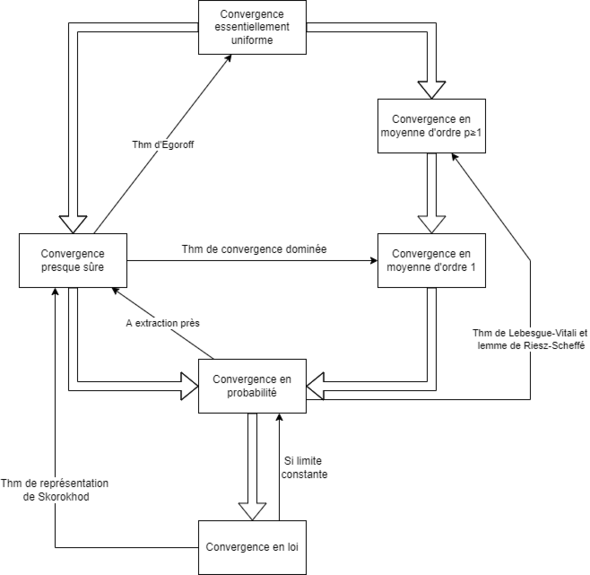
\includegraphics[scale=0.4]{figures/Cvg2va.png}
  \caption{Schéma résumant les liens entre convergences de variables (plus compliqué que celui donné en cours). La double flèche est une implication et la flèche simple est une implication dans certains cas.}
  \label{}
\end{figure}

\section{Convergence en loi}

\subsection{Fonction caractéristique}\marginnote{16-10-2023}

\begin{definition}
  Soit \((\Omega, \mathscr{A}, \mathbb{P})\) un espace probabilisé. On définit la fonction caractéristique de la variable aléatoire réelle \(X\) de la manière suivante :

  \[\varphi_t(X) = \mathbb{E}\left[e ^{itX}\right] = \int_{\Omega} e^{it X} d \mathbb{P}  = \int_{\mathbb{R}} e^{itx} d P_X(x).\]
\end{definition}

\begin{remark}[Cas particulier]
  Si \(X\) est à densité \(f _{X}(x)\), alors :

  \[\varphi _{X}(t) = \int_{\mathbb{R}} e^{itx} f_X(x)dx.  \]

  Il s'agit de la transformée de Fourier.
\end{remark}

\begin{prop}[Propriétés de la fonction caractéristique]

  \

  \begin{enumerate}
    \item \(\varphi_X\) est définie et continue \(\forall t \in \mathbb{R}\), en particulier elle est \textbf{uniformément continue}.
    \item \(\varphi _{aX+b}(t) = e^{itb}\varphi_X(at) \) ;
    \item Si \(\{ X_i \}_{i=1}^{\infty}\) sont indépendantes et on écrit \(S_n = \displaystyle \sum_{i=1}^{n}X_i\), alors
    \[\varphi _{X_n}(t) = \varphi _{X_1}(t)- \varphi _{X_n}(t).\]

    Si en plus les \(\{ X_i \}\) ont la même loi, alors

    \[\varphi _{S_n}(t) = \varphi _{X_1}(t) ^{n}.\]
  \end{enumerate}
\end{prop}

\begin{proof}

  \

  \begin{enumerate}
    \item Il faut que \(\varphi_X \in L ^{1}(\mathbb{P})\), i. e. \(\varphi_X \in L ^{1}(\mathbb{R}, P_X)\). Alors

    \[\int_{\Omega}^{} \left\lvert e^{itX}\right\rvert d \mathbb{P} = \int d \mathbb{P}=1.\]

    \item Montrons que \(\varphi_X\) est uniformément continue.

    On a

    \begin{gather*}
      \varphi_X(t) - \varphi_X(t_0) = \left\lvert \int_{}^{} \left(e^{itX} - e^{it_0 X}\right) \right\rvert = \int_{}^{} \left\lvert iX e^{i \xi X} \right\rvert  \left\lvert t-t_0 \right\rvert d \xi \\
      \leq \left\lvert t-t_0 \right\rvert \int_{}^{} \left\lvert X \right\rvert d \mathbb{P},
    \end{gather*}

    ce qui veut dire que la fonction est lipschitzienne, donc uniformément continue.

    \item On a

    \begin{gather*}
      \varphi _{S_n} = \int_{\Omega} e^{it}(X_1 + \dots + X_n) d \mathbb{P} = \int_{\Omega}^{} e^{itX_1} \dots e^{itX_n} d \mathbb{P} = \mathbb{E}[e^{itX_1}\dots e^{itX_n}] = \prod_{i=1}^{n} \mathbb{E}[e^{itX_i}] = \prod_{i=1}^{n} \varphi _{X_i}(t).
    \end{gather*}
  \end{enumerate}
\end{proof}

\begin{exemple}[Calculs des fonctions caractéristiques]

  \

  \begin{enumerate}
    \item \(X\) est une variable aléatoire binomiale \(B(n,p)\). On rappelle que

    \[\mathbb{P}(X=k) = C ^{k}_{n} p ^{k}(1-p)^{n-k}.\]

    Alors

    \begin{gather*}
      \varphi_X(t) = \int e^{itX} d \mathbb{P} = \int e^{itx} d P_X(x) = \sum_{k=0}^{n} e^{itk} C ^{k}_{n} p ^{k}(\underbrace{1-p}_{=q})^{n-k} =(q + p e^{it})^{n}.
    \end{gather*}

    \item \(X\) est de Bernoulli \(B(p)\), avec \(\mathbb{P}(X=1) = p\) et \(\mathbb{P}(X=0)=1-p\). Alors

    \begin{gather*}
      \varphi_X(t) = e^{it}p+q.
    \end{gather*}

    \item Variable de Gauss avec \(X\) qui a la loi \(\mathscr{N}(0,1)\).

    \begin{gather*}
      \varphi_X(t) = \frac{1}{\sqrt{ 2 \pi } }\int_{\mathbb{R}}^{} e^{itx} e^{-\frac{x ^2}{2}}dx = \frac{1}{\sqrt{ 2 \pi }} \int_{}^{} (\cos(tx)+ i \sin(tx)) e^{-\frac{x ^2}{2}}dx = \frac{1}{\sqrt{ 2 \pi } } \int_{\mathbb{R}} i \cos(tx) e^{-\frac{x ^2}{2}}dx,
    \end{gather*}

    car

    \begin{gather*}
      i \int_{}^{} \sin(tx) e^{- \frac{x ^2}{2}} dx = 0 \text{ (fonction impaire).}
    \end{gather*}

    %On intègre par parties :

    %\begin{gather*}
    %  \frac{1}{\sqrt{2\pi} \int_{\mathbb{R}} \cos(tx) e^{- \frac{x ^2}{2}} dx} = \frac{1}{\sqrt{2\pi}}
    %\end{gather*}
  %\end{enumerate}

  On dérive \(\varphi_X(t)\). Si

  \begin{gather*}
    \varphi_X(t) = \int_{\mathbb{R}} \cos(tx) e^{- \frac{x ^2}{2}}dx,
  \end{gather*}

  alors

  \begin{gather*}
    \varphi_X'(t) = \int_{\mathbb{R}} -x \sin(tx)e^{- \frac{x ^2}{2}} dx = \underbrace{\left[\sin(tx) e^{-\frac{x ^2}{2}} \right]_{-\infty}^{+\infty}}_{=0} - \int_{-\infty}^{+\infty} t \cos(tx)e^{-\frac{x ^2}{2}} dx = - t \varphi_X(t),
  \end{gather*}

  ce qui montre que \(\varphi_X'(t) = -t \varphi_X(t)\), i. e.

  \[\frac{d \varphi_X(t)}{dt} = - t \varphi_X(t).\]

  C'est une équation différentielle du premier ordre. On utilise la méthode des quadratures pour la résoudre. On a :

  \[\frac{d \varphi_X(t)}{\varphi_X(t)} = - t dt,\]

  ce qui donne, quand on intègre,

  \begin{gather*}
    \int_{\varphi_X(0)}^{\varphi_X(t)} \frac{d \varphi_X(t)}{\varphi_X(t)} = -\int_{0}^{t} t dt,
  \end{gather*}

  ce qui donne \(\ln(\varphi_X(t)) = - \displaystyle \frac{t ^2}{2}\), i. e. \(\varphi_X(t) = e^{- \frac{t ^2}{2}}.\)
\end{enumerate}
\end{exemple}

\begin{prop}
  Supposons que \(\mathbb{E}[\left\lvert X \right\rvert ^{n}] \less \infty\) (moment d'ordre \(n\) fini). Alors \(\varphi_X ^{(r)}(t)\) existe pour \(r \leq n\) où \(\varphi_X ^{(r)}\) dénote la dérivée d'ordre \(r\) de \(\varphi_X\) par rapport à \(t\) et :

  \begin{gather*}
    \varphi_X ^{(r)}(t) = \int_{\mathbb{R}} (ix)^{r} e^{itx} d P_X(x)
  \end{gather*}

  et

  \begin{gather*}
    \mathbb{E}[X ^{r}] = \frac{\varphi_X ^{(r)}(0)}{i ^{r}} \text{ pour } r \leq n.
  \end{gather*}

  De plus, on a :

  \begin{gather*}
    \varphi(t) = \sum_{k=0}^{n} \frac{(it)^{k}}{k!} \mathbb{E}[X ^{k}]+ \underbrace{\frac{(it)^{n}}{n!} \varepsilon_n(t)}_{\text{erreur}},
  \end{gather*}

  avec \(\left\lvert \varepsilon_n(t) \right\rvert \leq 3 \mathbb{E}[\left\lvert X \right\rvert ^{n}] \underset{t \to 0}{\longrightarrow} 0\).
\end{prop}

\begin{remark}
  Si \(\mathbb{E}[\left\lvert X \right\rvert ^{n}] \less \infty \implies \mathbb{E}[\left\lvert X \right\rvert ^{r}] \less \infty\), avec \(r \leq n\).
\end{remark}

\begin{proof}
  Soit \(n \geq  1\), on fait la preuve pour \(r=1\). On élimine l'indice \(X\) dans \(\varphi_X(t)\). On doit contrôler

  \begin{gather}
    \lim_{h \to 0} \frac{\varphi(t+h) - \varphi(t)}{h} = \lim_{h \to 0}  \frac{[e^{i(t+h)x}-e^{itx}  ]}{h}d P_X(t) = \int_{\mathbb{R}} \lim_{h \to 0} \left[\frac{e^{i(t+h)x} - e^{itx}}{h}\right] d P_X(x).  \label{lim_int}
  \end{gather}

  On développe la quantité \(e^{ix(t+h)}\) dans le point 0 :

  \begin{gather*}
    \frac{e^{ix(t+h)} - e^{itx}  }{h} = \frac{e^{ixt}+ e^{ixt}ixh+ O(h^2)- e^{itX}}{h} \approx e^{ixt}ix + O(h).
  \end{gather*}

  L'égalité \ref{lim_int} devient :

  \[\ref{lim_int} = \int_{\mathbb{R}} ix e^{itx} d P_X(x) \less \infty.\]

\end{proof}

\begin{thm}\marginnote{20-10-2023}
  Soient \(X\) et \(Y\) deux variables aléatoires telles que \(\varphi_X(t) = \varphi_Y, \forall t \in \mathbb{R}\). Donc \(P_X = P_Y\). \textbf{Les fonctions caractéristiques caractérisent complétement la loi}.
\end{thm}

\begin{thm}[\bsc{Formule d'inversion de Levy}]
  Soit \(X\) une variable aléatoire de fonction caractéristique

  \[\varphi_X(t) = \int_{\mathbb{R}} e^{itx}d P_X(x).\]

  Soient \(x\) et \(y\) deux points où la fonction de répartition \(F_X\) est continue. Alors

  \[F_X(b) - F_X(a) = \lim_{c \to +\infty} \frac{1}{2 \pi} \int_{-c}^{c} \frac{e^{-ita} - e^{-itb}}{it} \varphi_X(t)dt \text{ (intégrale impropre de Riemann).} \]
\end{thm}

On rappelle que la loi \(P_X\) est la mesure de Lebesgue-Stieltjes construite avec \(F_X\), i. e.

\[P_X((a,b]) = F_X(b)-F_X(a).\]

\begin{thm}
  Soit \(\varphi_X \in L ^{1}(\mathbb{R})\), i. e. \(\int_{\mathbb{R}} \left\lvert \varphi_X(t) \right\rvert dt \less \infty\). Alors la densité de \(X\) existe et

  \[f_X(x) = \frac{1}{2 \pi} \int_{\mathbb{R}} e^{itx} \varphi_X(t)dt.  \]
\end{thm}

\chapter{Convergence en loi}

\section{Convergence de mesures bornées sur \(\mathbb{R}^n\)}

On note \(\mathscr{M}\) l'ensemble de mesures positives sur \(\mathbb{R}^n\) muni de la tribu de \bsc{Borel}.

On note \(\mathscr{M}(b)\) l'ensemble de mesures de \(\mathscr{M}\) telles que si \(\mu \in \mathscr{M}(b)\), alors \(\mu(\mathbb{R}^n) \leq b\). Ce sont les mesures bornées par \(b\).

Enfin on note \(\mathscr{M}^{1}\) les mesures de probabilité \(\mu \in \mathscr{M}^{1}\) telle que \(\mu(\mathbb{R}^n) = 1\).

Avant de construire les topologies, on introduit deux classes de fonctions :

\begin{enumerate}
  \item \(\mathscr{C}_0(\mathbb{R}^n)\) qui sont les fonctions tendant vers 0 à l'infini, c'est-à-dire

  \[\forall \varepsilon \bg 0, \exists K _{\varepsilon} \text{ compact tel que } \left\lvert f(x) \right\rvert \less \varepsilon, \forall x \in (K _{\varepsilon})^{C}.\]
  \item \(\mathscr{C}_b(\mathbb{R}^n)\), l'ensemble des fonctions bornées :

  \[\forall x \in \mathbb{R}, \left\lvert f(x) \right\rvert \leq b.\]
\end{enumerate}

\begin{definition}
  Sur \(\mathscr{M}\) on définit deux topologies, \textsf{faible} et \texttt{étroite}. Il s'agit des deux topologies moins fines qui rendent continues les applications :

  \begin{gather*}
    \mu \longmapsto \int_{}^{} f d \mu, f \in \mathcal{C}_0(\mathbb{R}^n) \text{ (faible),} \\
    \mu \longmapsto \int_{}^{} d f \mu, f \in \mathscr{C}_b(\mathbb{R}^n) \text{ (étroite).}
  \end{gather*}
\end{definition}

Pour \(\mu_1, \mu_2 \in \mathscr{M}\), on définit

\[d(\mu_1, \mu_2) = \sum_{k=1}^{\infty} \frac{\left\lvert \int_{}^{} f_k d \mu_1 - \int_{}^{} f_k d \mu_2  \right\rvert}{2 ^{k}},\]

où \(\{ f_k \}\) est une suite dense dans \(\mathscr{C}_{0,b}(\mathbb{R}^n)\).

\subsection{Convergence}

\begin{definition}
  Prenons une suite \(\{ \mu_n \} \in \mathscr{M}\).

  On dira que \(\mu_n\) converge \textsf{faiblement} vers \(\mu \in \mathscr{M}\) si

  \[\lim_{n \to \infty} \int f d \mu_n = \int f d \mu, \forall f \in \mathscr{C}_0(\mathbb{R}^n).\]

  Elle converge \texttt{étroitement} si :

  \[\lim_{n \to \infty} \int f d \mu_n = \int f d \mu, \forall f \in \mathscr{C}_b(\mathbb{R}^n).\]
\end{definition}

\begin{remark}
  La convergence étroite implique la convergence faible.
\end{remark}

En probabilité, on utilisera surtout la convergence étroite.

\begin{prop}

  \

  \begin{enumerate}
    \item Sur \(\mathscr{M}^{1}\), les deux topologies co\"incident.
    \item \emph{``Théorème de Banach-Ailogu''} L'espace \(\mathscr{M}(b)\) est compact pour la topologie faible, c'est-à-dire toute suite de mesures bornées (par \(b\)) admet une sous-suite convergente faiblement vers une mesure \(\mu \in \mathscr{M}(b)\).
    \item Soit \(\{ \mu_n \}\) et \(\mu \in \mathscr{M}(b)\) telle que \(\mu_n \longrightarrow \mu\) faiblement. Alors la suite \(\{ \mu_n \}\) converge étroitement vers \(\mu\) si

    \[\lim_{k \to \infty} \mu_k(\mathbb{R}^n) = \mu(\mathbb{R}^n).\]

    La réciproque est aussi vraie.
  \end{enumerate}
\end{prop}

\begin{definition}\label{mu-cont}
  Soit \(\mu\) un élément de \(\mathscr{M}\). Un borélien \(A\) est appelé de \(\mu\)-continuité si

  \begin{gather*}
    \mu(\underset{\tiny\text{frontière}}{\partial A}) = 0.
  \end{gather*}
\end{definition}

\begin{thm}
  Soit \(\{ \mu_n \}_{n=1}^{\infty}\) une suite de mesures dans \(\mathscr{M}(b)\). Les deux assertions sont alors équivalentes :

  \begin{enumerate}
    \item \(\mu_n\) converge étroitement vers \(\mu\) ;
    \item Pour tout borélien \(A\) de \(\mu\)-continuité, on a
    \[\lim_{n \to \infty} \mu_k(A) = \mu(A).\]
  \end{enumerate}
\end{thm}

On va parler maintenant de la convergence en loi.

Soit \(\forall n \in \mathbb{N}\) une suite de variables aléatoires \(X_n\) définies sur les espaces \((\Omega_n, \mathscr{A}_n, \mathbb{P}_n)\). Soit \(X\) une autre variable aléatoire réelle à valeurs dans \(\mathbb{R}^{d}\) et définie sur \((\Omega, \mathscr{A}, \mathbb{P})\).

\begin{definition}
  La suite \(\{ X_n \}_{n=1}^{\infty}\) converge en loi (en distribution) vers \(X\) si la suite des lois \(P _{X_n}\) converge étroitement vers \(P_X\), et on écrira :

  \[P _{X_n} \stackrel{\mathscr{L}}{\longrightarrow} P_X.\]
\end{definition}

\begin{definition}
  Soit \(\{ X_k \}_{k=1}^{\infty}\)  une suite de variables aléatoires sur \((\Omega_k, \mathscr{A}_k, \mathbb{P}_k)\) et soit \(\mu\) une probabilité sur \(\mathbb{R}^{d}\). La suite \(\{ X_k \}_{k=1}^{\infty}\) converge étroitement vers \(\mu\) si la suite \(P _{X_n}\) converge étroitement vers \(\mu\) et on écrira

  \[X_n \stackrel{\mathscr{L}}{\longrightarrow} \mu.\]
\end{definition}

\begin{remark}
  Ici, on ne connaît pas forcément la variable aléatoire limite. On connaît seulement la distribution limite.
\end{remark}

\begin{thm}[Levy]
  A nouveau on a la suite \(\{ X_k \}_{k=1}^{\infty}\) avec \(X_k \in (\Omega_k, \mathscr{A}_k, \mathbb{P}_k)\).

  \begin{enumerate}
    \item \label{Levy1}Supposons que \(X_k\) converge en loi vers la variable aléatoire \(X\) définie sur \((\Omega, \mathscr{A}, \mathbb{P})\). Alors

    \[\lim_{k \to \infty} \varphi _{X_k}(t) = \varphi_X(t), \forall t \in \mathbb{R}.\]
    \item Supposons que \(\varphi _{X_k}(t)\) converge simplement (pour tout \(t \in \mathbb{R}\)) vers une fonction \(\varphi(t)\) qui est continue en 0. Alors \(\varphi\) est la fonction caractéristique d'une mesure de probabilité \(\mu\) et \(P _{X_n}\) converge étroitement vers \(\mu\), c'est-à-dire on a

    \[P _{X_k}\stackrel{\mathscr{L}}{\longrightarrow} \mu.\]

    En plus, il existe une variable aléatoire \(X\) \textbf{non unique} telle que

    \[X_k \stackrel{\mathscr{L}}{\longrightarrow} X.\]
  \end{enumerate}
\end{thm}

\begin{proof}\marginnote{23-10-2023}

  \

  \begin{enumerate}
    \item
      \begin{gather*}
        \varphi _{X_k}(t) = \int_{\mathbb{R}}^{} \underset{\substack{\text{continue} \\ \text{bornée}}}{e^{itx_k}} d P _{X_k}(x_k)  \underset{k \to +\infty }{\longrightarrow}  \int_{\mathbb{R}} e^{itx} d P_X(x).
      \end{gather*}

    \item On dénote \(P _{X_n} = P_n\). Par compacité, il existe une sous-suite \(n_k\) telle que \(P _{n_k} \longrightarrow \mu\), avec \(\mu\) une mesure bornée (\(\in \mathscr{M}(b)\)), et cette convergence est faible. L'objectif est de démontrer que \(\mu\) est une mesure de probabilité. On y arrive si on montre que

    \[\lim_{k \to +\infty} P _{n_k}(\mathbb{R}^d) = \mu(\mathbb{R}^d). \]

    Grâce à ce résultat-là, on montrera aussi que la convergence est étroite.

    \textbf{\emph{Astuce}} \ Soit \(\nu\) une mesure bornée quelconque et soit \(\varphi _{\nu}\) sa fonction caractéristique. On a

    \[\varphi _{\nu}(t) = \int_{\mathbb{R}^d} e^{itx} d \nu(x).\]

    On construit (pour \(\nu \bg 0\))

    \begin{gather*}
      \frac{1}{u} \int_{0}^{u} \varphi _{\nu}(t)dt = \frac{1}{u}\int_{0}^{u}\left(\int_{\mathbb{R}^d} e^{itx}d \nu(x)  \right) \stackrel{\text{Fubini}}{=} \frac{1}{u}\int_{\mathbb{R}} \left(\int_{0}^{u} e^{itx}dt  \right) d \nu(x)  = \frac{1}{u} \int_{\mathbb{R}} \frac{e^{ixu}-1 }{iux}d \nu(x).
    \end{gather*}

    On applique ces calculs à la mesure \(\mu\) :

    \begin{gather}
      \frac{1}{u} \int_{0}^{u} \varphi_\mu(t)dt = \int_{\mathbb{R}} \underbrace{\frac{e^{ixu}-1 }{iux}}_{\substack{\text{continue},\\\in \mathscr{C}_b(\mathbb{R}^d)}}d \mu(x)  = \lim_{k \to +\infty} \int_{\mathbb{R}^d} \frac{e^{iux}-1}{iux} d P _{n_k}  = \lim_{k \to+\infty} \frac{1}{u} \int_{0}^{u} \varphi_{P_{n_k}}(t)dt.  \label{equation45}
    \end{gather}

    On observe que \(\left\lvert \varphi_{P_{n_k}}(t) \right\rvert \leq \varphi _{P _{n_k}}(0) = 1\), donc on peut passer à la limite dans l'intégrale :

    \begin{gather*}
      \ref{equation45} = \frac{1}{u} \int_{0}^{u} \lim_{k \to \infty}  \varphi _{P _{n_k}}(t)dt = \frac{1}{u} \int_{0}^{u} \varphi(t)dt.
    \end{gather*}

    On a trouvé que

    \[\frac{1}{u}\int_{0}^{u} \underbrace{\varphi_\mu(t)dt}_{\substack{\text{cont. en 0} \\ \text{car fct car.}}} = \frac{1}{u} \int_{0}^{u} \underbrace{\varphi(t)}_{\substack{\text{cont. en 0}\\ \text{par hyp.}}}dt. \]

    Par le théorème de la valeur moyenne,

    \begin{gather*}
      \lim_{u \to 0}\frac{1}{u} \int_{0}^{u} \varphi_\mu(t)dt = \varphi_\mu(0),\\
      \lim_{u \to 0}\frac{1}{u} \int_{0}^{u} \varphi(t)dt = \varphi(0).
    \end{gather*}

    Il faut se rappeler qu'on doit montrer que \(\mu(\mathbb{R}^d) = 1\). En effet,

    \begin{gather*}
      \mu(\mathbb{R}^d) = \int_{\mathbb{R}^d}e^{i0x} d \mu(x) = \varphi_\mu(0) = \varphi(0) \stackrel{\text{hyp}}{=} \lim_{k \to \infty} \varphi _{P _{n_k}}(0) = \lim_{k \to \infty} \int_{\mathbb{R}^d} e^{i 0 x} d P _{n_k}(x) = 1.
    \end{gather*}

    Donc \(P _{n_k}\) converge aussi étroitement vers \(\mu\) (mesure de probabilité).

    \

    Par la première partie du théorème de Levy \ref{Levy1}, la convergence étroite de \(P _{n_k} \longrightarrow \mu\) entraîne que \(\varphi _{P _{n_k}}(t) \longrightarrow \varphi _{\mu}(t)\).

    \textbf{Mais} aussi \(\varphi _{P _{n_k}}(t) \longrightarrow \varphi(t)\). Donc on a établi que \(\varphi_\mu(t) = \varphi(t)\). Pour une autre sous-suite, on a \(\varphi _{P _{n_j}} \longrightarrow \varphi _{\mu'}(t) = \varphi(t)\).

    Donc toutes les fonctions caractéristiques correspondant à des \(\mu\) différentes sont \emph{égales}. Il y a une correspondance biunivoque entre \(\varphi\) et \(\mu\). On en déduit que toutes les ``\(\mu\)'' sont égales, ce qui implique que toutes les sous-suites qu'on peut engendrer à partir de \(P_n\) ont la même limite. On a ainsi montré que

    \[P_n \stackrel{\text{étroite}}{\longrightarrow} \mu.\]
  \end{enumerate}
\end{proof}

\textbf{\emph{Question}} \ \emph{Y a-t-il une variable aléatoire sur un certain espace probabilisé qui a \(\mu\) comme loi ?}

On prend \((\Omega, \mathscr{A}, \mathbb{P}) = (\mathbb{R}^d, \mathscr{B}(\mathbb{R}^d), \mu)\) et \(X : \Omega \longrightarrow \mathbb{R}^d\) est telle que \(X = \operatorname{id}\).

\begin{prop}
  Supposons que \(X_n \stackrel{\mathscr{L}}{\longrightarrow} X\) (en loi). Soit \(f\) une fonction continue de \(\mathbb{R}^d\) à valeurs dans \(\mathbb{R}\). Alors

  \[f(X_n) \stackrel{\prec}{\longrightarrow} f(x).\]
\end{prop}

\begin{thm}[La convergence en probabilité implique la convergence en loi]
  Soit \(\{ X_n \}\) une suite de variables aléatoires définies sur le même espace \((\Omega, \mathscr{A}, \mathbb{P})\) à valeurs dans \(\mathbb{R}^d\). Supposons que \(X_n\) converge en probabilité vers la variable aléatoire \(X\). Alors \(X_n\) converge aussi en loi vers \(X\).
\end{thm}

\begin{proof}
  Si l'on veut montrer que \(X_n \stackrel{\mathscr{L}}{\longrightarrow} X\), il suffit, pour \(f \in \mathscr{C}_b(\mathbb{R}^d)\), de montrer que

  \[\int_{}^{} f d P _{X_n} \underset{n \to +\infty}{\longrightarrow} \int_{}^{} f d P_X \text{ (étroite).}\]

  En effet,

  \begin{gather*}
    \left\lvert \int_{}^{} f d P _{X_n} - \int_{}^{} f d P_X   \right\rvert \stackrel{\text{transfert}}{=} \left\lvert \int_{\Omega}^{} f \circ X_n d \mathbb{P} - \int_{\Omega}^{} f \circ X_n d \mathbb{P}  \right\rvert = \left\lvert \int_{}^{} [f \circ X_n - f \circ X] d \mathbb{P}  \right\rvert \\
    = \int_{\{ \left\lvert f \circ X_n - f \circ X \right\rvert \bg \varepsilon \}} \left\lvert f \circ X_n - f \circ X \right\rvert d \mathbb{P} + \int_{\{ \left\lvert f \circ X_n - f \circ X \right\rvert \less \varepsilon\}} \left\lvert f \circ X_n - f \circ X \right\rvert d \mathbb{P} \\
    \leq \varepsilon + 2 \left\Vert f \right\Vert _{\infty} \underset{\longrightarrow 0 \text{ quand } n \longrightarrow \infty}{\mathbb{P}(\left\lvert f \circ X_n - f \circ X \right\rvert \bg \varepsilon)}.
  \end{gather*}
\end{proof}

%On envoie \(n \longrightarrow \infty\) et donc \(\mathbb{P}(\left\lvert f \circ X_n - f \circ X \right\rvert) \longrightarrow \infty\). On envoie après \(\varepsilon \longrightarrow 0\).


\begin{thm}
  Soit \(\{ X_n \}\) une suite de variables aléatoires toutes définies sur un même \((\Omega, \mathscr{A}, \mathbb{P})\) à valeurs dans \(\mathbb{R}^d\). Supposons que \(X_n \stackrel{\mathscr{L}}{\longrightarrow} \text{constante} =c\). Alors \(X_n \stackrel{\mathbb{P}}{\longrightarrow} c\).
\end{thm}

\begin{proof}
  \(\mu_n \stackrel{\mathscr{L}}{\longrightarrow} \mu\) si et seulement si pour tout borélien \(A\) de \(\mu\)-continuité, \(\mu_n(A) \longrightarrow \mu\).

  On sait que \(P _{X_n} \stackrel{\mathscr{L}}{\longrightarrow} \delta _{\{ c \}}\) (loi de la variable aléatoire limite \(X = c\)). On dénote avec \(B(c, \varepsilon)\) la boule fermée de centre \(c\) et de rayon \(\varepsilon\). On note que \(\delta _{\{ c \}}(\partial B(c, \varepsilon)) = 0\). Donc \(B(c, \varepsilon)\) est un ensemble de \(\delta _{\{ c \}}\)-continuité. Donc par la définition \ref{mu-cont}, on sait que

  \[\lim_{n \to \infty} P _{X_n}(B(c, \varepsilon)) = \delta _{\{ c \}}(B(c,\varepsilon))=1,\]

  donc

  \[\lim_{n \to \infty} P_X(x, \left\lvert x-c \right\rvert \bg \varepsilon) = 0.\]
\end{proof}

\begin{exemple}
  Sur \((\Omega, \mathscr{A}, \mathbb{P})\) on a une variable aléatoire de Bernoulli \(X\) de paramètre \(\displaystyle\frac{1}{2}\). On pose \(X_n = X\). On a que \(X_n \stackrel{\mathscr{L}}{\longrightarrow} X\). On considère \(Y = 1 - X\). Elle est encore de Bernoulli de paramètre \(\displaystyle \frac{1}{2}\) et \(X_n \stackrel{\mathscr{L}}{\longrightarrow} Y\). Montrer que \(X_n\) ne converge pas en probabilité vers \(Y\).
\end{exemple}

\begin{proof}
  \(\forall f \in \mathscr{C}_b,\) on doit montrer que \(\int f d P _{X_n} \longrightarrow \int f d P_Y\). On a

  \[\underbrace{f(0) \frac{1}{2}+ f(1) \frac{1}{2}}_{X} = \underbrace{f(1)\frac{1}{2} + f(0)\frac{1}{2}}_{Y}, \]

  donc \(X_n\) converge en probabilité vers \(Y\).

  On a

  \begin{gather*}
    \mathbb{P}(\left\lvert X_n - Y \right\rvert \bg \varepsilon) = \mathbb{P}(\left\lvert X - Y \right\rvert \bg \varepsilon) = \mathbb{P}(\left\lvert X - 1 + X \right\rvert \bg \varepsilon) = \mathbb{P}(\left\lvert 2 X - 1 \right\rvert \bg \varepsilon).
  \end{gather*}

  On a \(\mathbb{P}(\left\lvert 2 X -1  \right\rvert =1) = 1\), donc \(X_n\) ne converge pas en probabilité vers \(Y\).
\end{proof}

\begin{thm}
  Soit \(\{ X_n \}\) une suite de variables aléatoires définies sur des espaces \((\Omega_n, \mathscr{A}_n, \mathbb{P}_n)\) avec chacune une fonction de répartition \(F _{X_n}\). Soit \(X\) une autre variable aléatoire définie sur \((\Omega, \mathscr{A}, \mathbb{P})\) avec fonction de répartition \(F_X\). La suite \(\{ X_n \}\) converge en loi vers \(X\) si et seulement si \(F _{X_n}(t)\) converge vers \(F_X(t)\) dans les points de continuité de cette dernière.
\end{thm}

\begin{proof}

  \

  \begin{enumerate}
    \item \emph{Partie nécessaire.} On suppose que \(X_n \stackrel{\mathscr{L}}{\longrightarrow} X\). Soit \(t\) un point où \(F_X\) est continue. On veut montrer que \(F _{X_n}(t) \longrightarrow F_X(t)\).

    Prenons l'ensemble \((-\infty, t]\). Cet ensemble-là est de \(P_X\)-continuité, car

    \begin{gather*}
      P_X(\{ t \}) = F_X(t) - F_{X-0}(t)=0.
    \end{gather*}

    Donc

    \[\lim_{n \to \infty} F _{X_n}(t) = \lim_{n \to \infty} P _{X_n}((-\infty, t]) = P_X((-\infty, t]) = F_X(t).\]

    \item \emph{Partie suffisante.} Par hypothèse, \(F _{X_n}(t) \longrightarrow F_X(t)\) et \(F _{X_n}\) est continue en \(t\). On va montrer que \(X_n \stackrel{\mathscr{L}}{\longrightarrow} X\).

    On sait que les points où \(F_X\) n'est pas continue sont au plus dénombrables. Etant donné \(f \in \mathscr{C}_b(\mathbb{R})\), on introduit une fonction en escalier \(g : \mathbb{R} \longrightarrow \mathbb{R}\) de type

    \[g(x) = \sum_{j=1}^{n} \alpha_j \mathds{1}_{[a_j, b_j]}, a_j \less b_j \leq a _{j+1} \less b _{j+1} \]

    et les points \(\{ a_j, b_j \}\) sont de continuité par \(F_X\) et en plus

    \[\left\Vert F_X(t)-g(t) \right\Vert_{\infty} \less \varepsilon. \]

    On a

    \begin{gather*}
      \int_{\mathbb{R}} g(t) d P _{X_n}(t) = \sum_{j=1}^{k} \alpha_j P _{X_n}([a_j,b_j]) = \sum_{j=1}^{k} \alpha_j [F(b_j)-F(a_j)].
    \end{gather*}

    On a alors :

    \begin{gather*}
      \lim_{n \to \infty} \int_{\mathbb{R}}^{} g(t) d P _{X_n}(t) = \lim_{n \to \infty} \sum_{j=1}^{k} \alpha_j[F _{X_n}(b_j) - F _{X_n}(a_j)] \\
      = \sum_{j=1}^{k} \alpha_j[F_X(b_j)- F_X(a_j)] = \int_{\mathbb{R}}^{}g(t)d P_X(t).
    \end{gather*}

    Soit \(f \in \mathscr{C}_b(\mathbb{R})\). On écrit

    \begin{gather*}
      \left\lvert \int_{}^{}f d P _{X_n} - \int_{}^{}f d P_X   \right\rvert \leq \left\lvert \int_{}^{}(f-g)d P _{X_n}  \right\rvert + \left\lvert \int_{}^{}g d P _{X_n} - \int_{}^{}g d P_X   \right\rvert + \left\lvert \int_{}^{} (g-f)d P_X  \right\rvert \\
      \leq  2 \left\Vert f-g \right\Vert _{\infty} + \left\lvert \int g d P _{X_n}- \int_{}^{} g d P_X  \right\rvert \leq 2 \varepsilon + \left\lvert \int_{}^{} g d P _{X_n} - \int g d P_X  \right\rvert.
    \end{gather*}
  \end{enumerate}
\end{proof}

\begin{lemma}[De Schiffe, pour les variables à densité]
  Soit \(\{ X_n \}\) une suite de variables aléatoires définies sur \((\Omega, \mathscr{A}_n, \mathbb{P}_n)\) et avec des densités \(f _{X_n}\). Si la suite \(f _{X_n}\) converge Lebesgue-presque partout vers une fonction \(f\) telle que \(\displaystyle\int f d \operatorname{Leb}\) est croissante, alors la suite \(X_n\) converge en loi vers la mesure \(f d \operatorname{Leb}\).
\end{lemma}

\subsection{Variables discrètes}

\begin{prop}
  Soit \(\{ X_n \}\) suite de variables discrètes sur le même espace \((\Omega, \mathscr{A}, \mathbb{P})\) à valeurs dans \(\mathbb{Z}\). On a l'équivalence entre les assertions suivantes :

  \begin{enumerate}
    \item \(X_n \stackrel{\mathscr{L}}{\longrightarrow} X\) ;
    \item \(\displaystyle \lim_{n \to \infty} \mathbb{P}(\underset{r \in \mathbb{Z}}{X_n = r}) = \mathbb{P}(X=r)\).
  \end{enumerate}
\end{prop}

\begin{thm}[Central limite]\marginnote{ \ {\fontencoding{U}\fontfamily{futs}\selectfont\char 66\relax}}
  Soit \(\{ X_n \}\) une suite de variables aléatoires indépendantes et de même loi et de classe \(L ^2(\mathbb{P})\). Posons \(\mu = \mathbb{E}[X_1]\), \(\sigma ^2 = \mathbb{V}(X_1) \ (0 \less \sigma)\). Soit \(S_n = \displaystyle \sum_{j=1}^{n} X_j\). On écrit :

  \[\frac{S_n - \mu_n}{\sigma \sqrt{n}} = \frac{\sum_{j=1}^{n} X_j - n \mu}{\sigma \sqrt{n} }.\]

  Alors

  \[\mathbb{P}\left(\frac{S_n - \mu n}{\sigma \sqrt{n} } \leq t \right) = \frac{1}{\sqrt{ 2 \pi \sigma}} \int_{-\infty}^{t} e^{- \frac{1}{2}\left(\frac{x - \mu}{\sigma}\right)^2} dx.\]

  On aura

  \[\frac{S_n - \mu n}{\sigma \sqrt{n}} \stackrel{\mathscr{L}}{\longrightarrow} \mathscr{N}(\mu, \sigma ^2).\]
\end{thm}

\begin{proof}
  On introduit

  \begin{gather*}
    \overline{X_n} = \frac{X_n}{n} = \frac{1}{n} \sum_{j=1}^{n} X_j, \\
    Y_n = \frac{S_n - \mu n}{\sigma \sqrt{n}} = \frac{\overline{X_n}-\mu}{\frac{\sigma}{\sqrt{n}}}.
  \end{gather*}

  Considérons la variable centrée \(X_n - \mu = X_1 - \mu\). On a

  \begin{gather*}
    \varphi _{X_1 - \mu}(t) = 1 - \frac{t ^2 \sigma ^2}{2} + o(t ^3).
  \end{gather*}

  L'espérance de \(X_1 - \mu\) est nulle. La variance de \(X_1\) est \(\sigma ^2\).

  On a

  \begin{gather*}
    Y_n = \frac{\sum_{j=1}^{n}(X_j - \mu)}{\sigma \sqrt{n}}.
  \end{gather*}

  La fonction caractéristique de cette variable vaut :

  \begin{gather*}
    \varphi _{Y_n}(t) = \varphi _{X_1 - \mu} \left(\frac{t}{\sigma \sqrt{n}}\right)^{n} = \left[1 - \frac{1}{2} \frac{\sigma ^2 t ^2}{\sigma ^2 n} + o(t ^2)\right] = \left[1 - \frac{1}{2}\frac{t ^2}{n} + o(t ^2)\right] \longrightarrow e^{- \frac{t ^2}{2}}.
  \end{gather*}
\end{proof}

\chapter{Variables gaussiennes}\marginnote{27-10-2023}

\section{Généralités}

Soit \(X ^{T} = (X_1, \dots, X_n)\) (transposée) un vecteur aléatoire, avec \(X_1, \dots, X_n\) définies sur le même espace \((\Omega, \mathscr{A}, \mathbb{P})\).

\begin{definition}
  On dira que le vecteur \(X = (X_1, \dots, X_n)\) est gaussien (vecteur aléatoire gaussien, VAG) si toute combinaison linéaire des \(X_i, i \in \{1, \dots, n \}\) est une variable gaussienne.

  Donc en particulier, chaque \(X_i\) est une variable gaussienne.
\end{definition}

\begin{definition}[Rappel : variable gaussienne]
  Une variable \(Y\) est dite gaussienne si c'est une variable à densité, et la densité a la forme suivante :

  \[f(x) = \frac{1}{\sqrt{2 \pi \sigma}} e^{-\frac{1}{2}\left(\frac{x-m}{\sigma}\right)^2},\]

  où \(m = \mathbb{E}[Y]\) et \(\sigma ^2 = \mathbb{V}(Y)\).
\end{definition}

On utilisera souvent la gaussienne standart de loi \(\mathscr{N}(0,1)\), dans ce cas on aura

\[f(y) = \frac{1}{\sqrt{2 \pi}} e^{-\frac{y ^2}{2}}.\]

\emph{L'objectif est de trouver la loi du vecteur, \(P _{X_1, \dots, X_n}(x_1, \dots,x_n)\) et de savoir si elle est à densité. On veut aussi savoir s'il existe un critère d'indépendance des \(\{ X_i \}_{i=1}^{n}\). Enfin, on cherchera à calculer la fonction caractéristique de \(X\).}

\section{Fonctions caractéristiques}

Pour la gaussienne standart, la fonction caractéristique est

\[\varphi_Y(t) = e^{-\frac{1}{2} t ^2}.\]

Dans le cas général, la fonction caractéristique se calcule comme suit :

\[\varphi_Y(t) = e^{itm}e^{- \frac{1}{2}\sigma ^2 t ^2}.\]

\begin{prop}
  La fonction caractéristique du vecteur gaussien \(X\) se calcule de la façon suivante :

  \begin{gather*}
    \varphi _{X_1, \dots,X_n}(t_1, \dots, t_n) = \int e^{i[t_1 X_1 + \dots + t_n X_n]}d \mathbb{P} = \int e^{i (t,X)}d \mathbb{P}\\
    \stackrel{\text{transfert}}{=}\int e^{i(t,X)}d P_X(x_1, \dots, x_n) = \int e^{it Y} d \mathbb{P} = \varphi_Y(1) = e^{im}e^{-\frac{1}{2}\sigma ^2},
  \end{gather*}

  où \(Y = \displaystyle\sum_{i=1}^{n} t_i X_i\). C'est une variable gaussienne. Lorsqu'on introduit \(Y\), on fait les calculs comme si c'était une variable gaussienne. On rappelle que \(m= \mathbb{E}[Y], \sigma ^2 =\mathbb{V}(Y)\).
\end{prop}

\begin{remark}
  \((t_1, \dots, t_n)\) est le vecteur ligne tandis que \(\begin{pmatrix}
    X_1 \\
    \vdots \\
    X_n
  \end{pmatrix}\) est le vecteur colonne. \((t,X)\) est le produit scalaire euclidien.
\end{remark}

\begin{remark}
  L'espérance de \(Y\) est facile à calculer. En effet,

  \begin{gather*}
    m = \mathbb{E}[Y] = \mathbb{E}\left[\sum_{j=1}^{n} t_j X_j \right] = \sum_{j=1}^{n}t_i \mathbb{E}[X_j] = (t,M_X),
  \end{gather*}

  avec \(M_X = \begin{pmatrix}
  \mathbb{E}[X_1] \\
  \vdots \\
  \mathbb{E}[X_n]
  \end{pmatrix}\).

  On a de plus

  \begin{gather*}
    \sigma_Y ^2 \mathbb{V}(Y) = \mathbb{E}[(Y - \mathbb{E}[Y])^2] = \mathbb{E}\left[\sum_{j=1}^{n} \{ t_j X_j - t_j m _{X_j} \}^2\right] = t  \Sigma_{X} t ^{T},
  \end{gather*}

  où \(\Sigma_{X}\) est la matrice de dispersion. On la calcule ainsi

  \[\Sigma_X = \begin{pmatrix}
  \sigma _{X_1 X_1} & \dots & \sigma _{X_1 X_n} \\
  \vdots & \ddots & \vdots \\
  \sigma _{X_n X_1} & \dots & \sigma _{X_n X_n},
  \end{pmatrix}\]

  où \(\sigma _{X_i X_j} = \operatorname{Cov}(X_i X_j) = \mathbb{E}[X_i X_j] - \mathbb{E}[X_i]\mathbb{E}[X_j]\). Les éléments diagonaux de la matrice \(\Sigma_X\) sont en fait les variances de \(X_1, \dots, X_n\). C'est une matrice \textbf{symétrique}.

  On peut écrire de manière plus concise \(m_Y = t \cdot M_X\) et \(\sigma_Y ^2 = t \Sigma_X t ^{T}\).
\end{remark}

Le calcul de la fonction caractéristique devient donc

\begin{gather*}
  \varphi _{X_1, \dots, X_n}(t_1, \dots, t_n) = \varphi_Y(1) = e^{im_Y}e^{-\frac{1}{2}\sigma_Y ^2} = e^{it m_X} e^{-\frac{1}{2}t \Sigma_X t ^2}.
\end{gather*}

\

On suppose que \(\Sigma_X\) est \textbf{inversible} (critère de non-dégénérescence). On sait que \(\Sigma_X\) est symétrie et positive, elle est donc diagonalisable, c'est-à-dire il existe une matrice \(A\) inversible telle que

\[A ^{-1} \Sigma_X A = \operatorname{Id} = \begin{pmatrix}
  1 & \dots & 0 \\
  \vdots & \ddots & \vdots \\
  0 & \dots & 1
\end{pmatrix} (?????)\]

On fait un changement de variable \(Z = A ^{-1}(X - m_X)^{T} = (z_1, \dots, z_n)^{T}\). La matrice de dispersion de \(Z\) est donnée par

\[\Sigma_Z = A ^{-1} \Sigma_X A = \operatorname{Id}.\]

La fonction caractéristique de \(Z\) est donc

\[\varphi_Z(t) = e^{-\frac{1}{2}t \Sigma_Z}t ^{T} = e^{-\frac{1}{2}t t ^{T}} = \prod_{i=1}^{n} e^{-\frac{1}{2}t_j ^2} = \prod_{i=1}^{n} \varphi _{Z_i}(t).\]

\begin{prop}
  \(Z_1, \dots, Z_n\) sont indépendantes si et seulement si les fonctions caractéristiques se factorisent, autrement dit

  \[\varphi _{Z_1 \dots Z_n}(t_1, \dots, t_n) = \varphi _{Z_1}(t_1) \dots \varphi _{Z_n}(t_n).\]
\end{prop}

Observons que l'on a les densités de \(Z_1, \dots, Z_n\), à savoir \(f_Z(z_i) = \displaystyle \frac{1}{\sqrt{2 \pi}} e^{-\frac{z_i ^2}{2}}\).

Donc

\begin{gather*}
  f _{Z_1 \dots Z_n}(z_1, \dots, z_n) = \prod_{j=1}^{n} \frac{1}{\sqrt{2 \pi}} e^{-\frac{z_i ^2}{2}} = \frac{1}{(2 \pi) ^{\frac{n}{2}}} e^{-\frac{1}{2}z z ^{T}},
\end{gather*}

avec \(Z = (z_1, \dots, z_n)\). On remplace \(Z\) avec \(X\). La densité de \(X\) est égale à

\begin{gather*}
  f _{X_1 \dots X_n}(x_1, \dots, x_n) = \frac{1}{(2 \pi)^{\frac{n}{2}} \operatorname{det}(\Sigma_X)^{\frac{1}{2}}} e^{- \frac{1}{2}[(x- m_X)\Sigma_X ^{-1} (x-m_X)^{T}]}.
\end{gather*}

\begin{prop}
  Un vecteur gaussien est indépendant si et seulement si il est non-corrélé.
\end{prop}


%%%%%%%%%%%%%%%%%%%%%%%%%%%%%%%%%%%
%%%%%%%%%%%%%%%%%%%%%%%%%%%%%%%%%%%
%%%%%%%%%%%DENOMBREMENT%%%%%%%%%%%%
%%%%%%%%%%%%%%%%%%%%%%%%%%%%%%%%%%%
%%%%%%%%%%%%%%%%%%%%%%%%%%%%%%%%%%%

\chapter*{Dénombrement}
\addcontentsline{toc}{chapter}{Dénombrement}

\marginnote{15-09-2023}

On a 3 objets $\{ a,b,c \} $.
\section{Dispositions sans répétition}

\begin{tabular}{|c|c|c|}
  \hline
  Eléments & Combinaisons sans ordre & Combinaisons avec ordre \\
  \hline
  1 à 1 & $\{ a \}, \{ b \}, \{ c \} $ & $\{ a \}, \{ b \}, \{ c \} $ \\
  \hline
  2 à 2 & $\{ a,b \}, \{ a,c \}, \{ b,c \} $ & $\{ a,b \}, \{ b,a \}, \{ a,c \}, \{ c,a \}, \{ b,c \}, \{ c,b \} $ \\
  \hline
  3 à 3 & $\{ a,b,c \} $ & $\{ a,b,c \}, \{ a,c,b \}, \{ b,a,c \}, \{ c,a,b \}, \{ c,b,a \}, \{ b,c,a \} $ \\
  \hline
\end{tabular}

\section{Dispositions avec répétition}

\begin{tabular}{|c|c|c|}
  \hline
  Eléments & Dispositions sans ordre & Dispositions avec ordre \\
  \hline
  1 à 1 & $\{ a \}, \{ b \}, \{ c \} $ & $\{ a \}, \{ b \}, \{ c \} $ \\
  \hline
  2 à 2 & $\{ a,a \}, \{ b,a \}, \{ b,b \}, \{ a,c \}, \{ b,c \}, \{ c,c \} $ & $ \{ a,a \}, \{ a,b \}, \{ b,a \}, \{ b,b \}, \{ a,c \}, \{ c,a \}, \{ b,c \}, \{ c,b \} \{ c,c \} $ \\
  \hline
  3 à 3 & $\{ a,a,a \}, \{ a,a,c \}, \dots $ (10 éléments) & $\{ a,a,a \}, \{ a,a,c \}, \{ a,c,a \}, \{ c,a,a \}, \dots $ ($3 ^3 = 27$ éléments) \\
  \hline

\end{tabular}

\begin{figure}[h!]
  \centering
  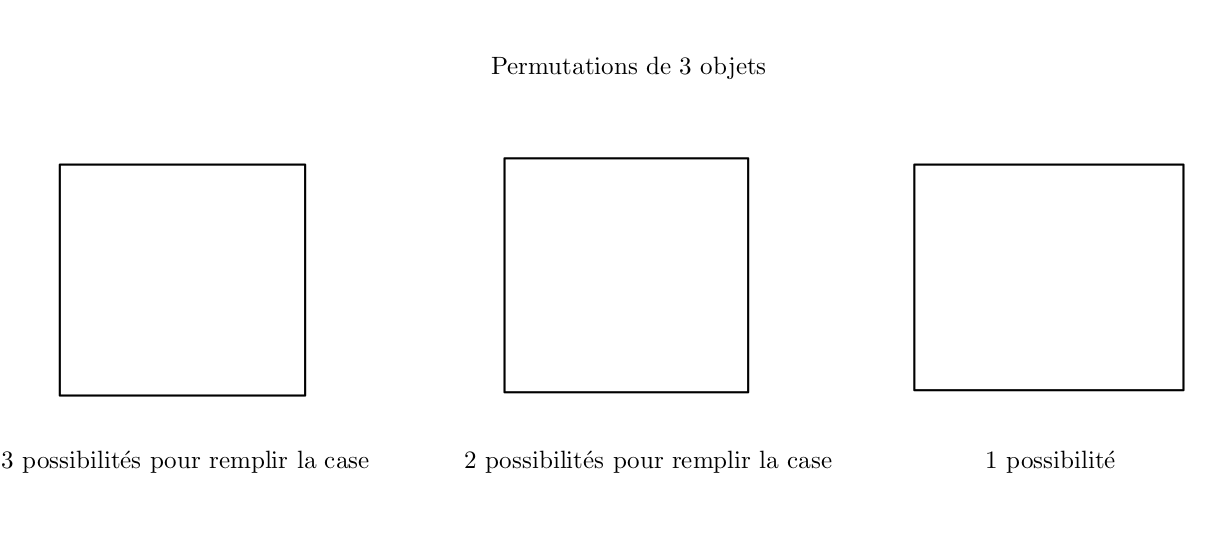
\includegraphics[scale=0.3]{figures/perm3.png}
  \caption{Permutations dans le cas de 3 objets (dispositions sans répétition et avec ordre)}
  \label{}
\end{figure}

\paragraph{Arrangements de $n$ objets pris $k$ à $k$ (dispositions avec ordre et sans répétition)} %(dans notre cas 3 objets pris 2 à 2)

Si on a 4 objets pris 2 à 2 : $\{ a,b,c,d \} $.

Si $a$ et $b$ sont fixés, alors $\{ a,b \} $ engendrera $\{ a,b,c,d \} $ et $\{ a,b,d,c \} $.

On a $$A _{n} ^{k} = \frac{n!}{(n-k)!}$$

\paragraph{Combinaisons de $n$ objets pris $k$ à $k$ (dispositions sans ordre et sans répétition)}

\begin{equation}
  C _{n} ^{k} = \frac{n!}{k!(n-k)!} = \binom{n}{k}.
\end{equation}

En fait,
\begin{equation*}
  C _{n} ^{k} = \frac{A _{n} ^{k}}{k!},
\end{equation*}

avec $k!$ le nombre de permutations des $k$ éléments.

%\paragraph{(combinaisons avec ordre et avec répétition)}

%\paragraph{(combinaisons sans ordre et avec répétition)}

Si on a $n$ objets à combiner $k$ à $k$ avec répétition, mais sans ordre, il y a

\begin{equation}
  C _{k} ^{n+1-k} = \frac{(n+1-k)!}{k!(n-1)!} \text{ combinaisons possibles.}
\end{equation}


%\begin{exo}
%  Dans une bibliothèque, il y a $n$ livres sur une étagère repartis au hasard. Parmi ces $n$ livres, $k$ sont d'un même auteur $A$, les autres d'auteurs différents. Calculer la probabilité qu'au moins $p$ livres de $A$ se retrouvent côte à côte dans les cas suivants :
%  \begin{enumerate}
%    \item $n=20, k=3, p=3$ ;
%    \item $n=20, k=5, p=2$ (\textbf{au moins} 2 livres).
%  \end{enumerate}
%\end{exo}


\section{Tirage des urnes sans remise}

$N$ boules de type $N_a, N_b$ tels que $N_a + N_b = N$.

On tire $n \less N$ boules.

Soit $E$ l'événement suivant : $\{ k \text{ boules parmi } n \text{ sont de type } a \}$.

Calculer la probabilité de $E$.

\begin{gather*}
  \mathbb{P}( E ) = \frac{C _{N_a} ^{k} C _{N_b} ^{n-k}}{C_N ^{n}} \text{ (formule hypergéométrique).}
\end{gather*}

\begin{proof}
  $\Omega = \text{ combinaisons de } N \text{ objets pris } n \text{ à } n \text{ sans les répéter. }   $

  On a $\sharp(\Omega) = C_N ^{n}$.

  Cas favorables : $C _{N_a} ^{k} C _{N_b}^{n-k}$.
\end{proof}

Cette formule est utilisée pour calculer la probabilité de gagner au loto. On a une grille de 49 numéros et on tire 6 numéros.

$N_a =$ les 6 numéros cochés par le joueur, $N_b = 49-6 = 43$ et $n=N_a$.

\begin{gather*}
  \mathbb{P}( \text{avoir 3 numéros gagnants} ) = \frac{C^{3}_{6} C^{3}_{43}}{C^{6}_{49}} \approx 0.018 \\
  \mathbb{P}( \text{avoir 6 numéros gagnants} ) = \frac{C^{6}_{6} C^{0}_{43}}{C_{49}^{6}} \approx 7,15 \times 10 ^{-8}.
\end{gather*}

\section{Tirage des urnes avec remise}

$N$ boules, $N_a$ de type $a$, $N_b$ de type $b$. On en tire $n$ (avec $n$ quelconque) et

\begin{equation*}
  E = \{ k \text{ boules parmi les } n \text{ tirées sont de type } a  \}.
\end{equation*}

On a $\sharp(\Omega) = N ^{n}$.

Cas favorables : $N_a ^{k} N_b ^{n-k} \binom{n}{k}$.

Donc

\begin{equation*}
  \mathbb{P}( E ) = \frac{N_a ^{k} N_b ^{n-k} \binom{n}{k}}{N ^{n}} = \frac{N_a ^{k} N_b ^{n-k} \binom{n}{k}}{N ^{k} N ^{n-k}} = \left( \frac{N_a ^{k}}{N}\right) ^{k} \left( \frac{N_b}{N}\right) ^{n-k} \binom{n}{k} = p_a ^{k} p_b ^{n-k} \binom{n}{k},
\end{equation*}

où $p_a$ et $p_b$ sont les pourcentages de $a$ et de $b$.

Il s'agit de la \textbf{loi binomiale}.

%%%%%%%%%%%%%%%%%%%%%%%%%%%%%%%%%%%%%%%%%%%%%%%%%%%%%%%%%%%%%%%%%%%%%%%%%%%%%%%%%%%%%%%%%%%%%%%%%%%%%%%%%%%%

\chapter*{Travaux dirigés}
\addcontentsline{toc}{chapter}{Travaux dirigés}

Dans ce document, vous ne trouverez que les énoncés des exercices, les corrections étant manuscrites. La numérotation dans les feuilles manuscrites correspond à celle dans ce document.

\begin{exo}
  Dans une bibliothèque, il y a $n$ livres sur une étagère repartis au hasard. Parmi ces $n$ livres, $k$ sont d'un même auteur $A$, les autres d'auteurs différents. Calculer la probabilité qu'au moins $p$ livres de $A$ se retrouvent côte à côte dans les cas suivants :
  \begin{enumerate}
    \item $n=20, k=3, p=3$ ;
    \item $n=20, k=5, p=2$ (\textbf{au moins} 2 livres).
  \end{enumerate}
\end{exo}

\begin{proof}

  \

  \begin{enumerate}
    \item

    \begin{figure}[h!]
      \center\addcontentsline{toc}{chapter}{Travaux dirigés}ing
      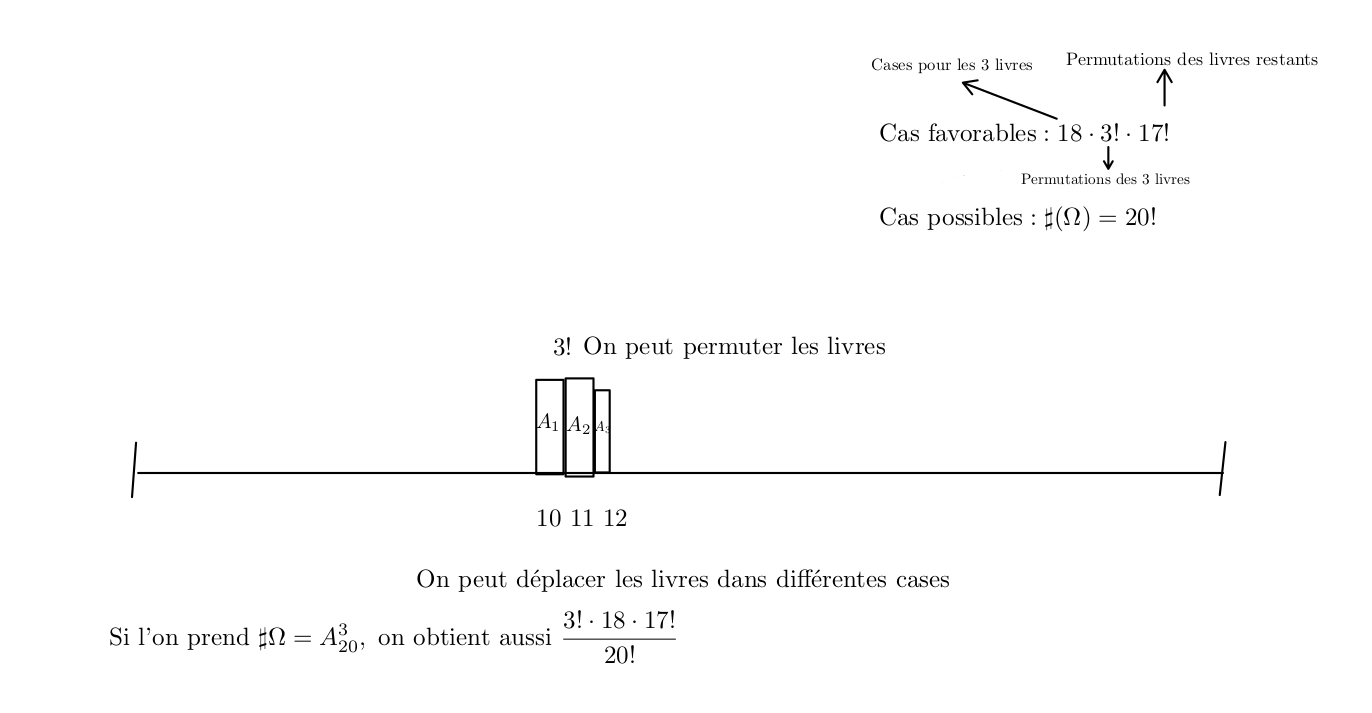
\includegraphics[scale=0.3]{figures/exo_livres.png}
      \caption{Solution pour (1)}
      \label{}
    \end{figure}

    %\item On note $E$ l'événement ``au moins 2 livres se trouvent côte à côte''. Notons $E ^{C}$ = ``il n'y a pas de livres de $A$ côte à côte''.
  \end{enumerate}
\end{proof}

\begin{exo}
  On lance 10 fois une pièce de monnaie. Calculer la probabilité qu'au cinquième lancer on obtient pile en sachant que le nombre total des piles obtenus est 3.
\end{exo}

\begin{exo}
  On a deux variables aléatoires \(X_1\) et \(X_2\) de même densité \(f(x) = \frac{1}{X ^2} \mathds{1}_{[1, \infty)}(x)\) et elles sont indépendantes. On pose
  \begin{gather*}
    U = X_1 X_2 \\
    V = \frac{X_1}{X_2}.
  \end{gather*}

  \begin{enumerate}
    \item Calculer la loi du couple \((U,V)\).
    \item \(U \text{ et } V \) sont-elles indépendantes ?
  \end{enumerate}
\end{exo}

\begin{exo}
  On place six boules de manière aléatoire et indépendante dans 3 boîtes. Calculer la probabilité que la première boîte contienne deux boules.
\end{exo}

\begin{exo}
  Un robinet a été installé le jour \(J\) et il fuit, les fuites se produisent chaque heure de manière indépendante et avec la probabilité \(p\).

  \begin{enumerate}
    \item Calculer la loi de la variable aléatoire \(F\) égale au nombre de fuites qui se sont produites tout au long de la journée (en 24 heures), ie \(\mathbb{P}(F=k), k \in \{ 0, \dots, 24 \}\).
    \item On dénote \(T(1)\) la variable aléatoire égale à l'heure de la première fuite. Calculer la loi de \(T(1)\), ie \(\mathbb{P}(T(1) = k), k=1, \dots, 24\).
    \item On dénote \(T(2)\) la variable aléatoire égale à l'heure de la deuxième fuite. Montrer que \(T(1)\) et \(T(2)-T(1)\) sont indépendantes et ont la même loi.
  \end{enumerate}
\end{exo}

\begin{exo}
  Sur l'espace probabilisé \((\Omega, \mathscr{A}, \mathbb{P})\), on considère le vecteur aléatoire \((X, Y)\) à valeurs dans \(\mathbb{R}^2\) et de loi \(P_X\) à densité

  \[f _{XY}(x,y) = \alpha(1-x ^2) \mathds{1}_{[0, 1]}(x)y e^{-3y} \mathds{1}_{[0, \infty)}(y), \]

  où \(\alpha \in \mathbb{R}\).

  \begin{enumerate}
    \item Déterminer \(\alpha\).
    \item Déterminer les lois marginales.
    \item Calculer \(\mathbb{P}(0 \less X \leq 2, Y \geq 1)\).
    \item Calculer la matrice de dispersion \(D\) de \((X,Y)\):

    \[D= \left(\begin{matrix}
      \mathbb{V}(X) & \operatorname{Cov}(X,Y) \\
      \operatorname{Cov}(Y,X) & \mathbb{V}(Y)
    \end{matrix}\right).\]
  \end{enumerate}


\end{exo}

\begin{exo}
  Soient \(X\) et \(Y\) deux variables aléatoires indépendantes et de même loi \(e^{-x}\mathds{1}_{[0, \infty)}(x)\). Déterminer la loi conjointe des nouvelles variables \(U = X+Y\) et \(V = \displaystyle\frac{X}{X+Y}\) et montrer que \(V\) a une loi uniforme sur \([0,1]\).
\end{exo}

\begin{exo}
  Soient \(X\) et \(Y\) deux variables aléatoires dont \(Y\) est de densité \(f _{Y}(y)\) et posons \(Z = X+Y\).

  \begin{enumerate}
    \item Prenons \(X\) et \(Y\) indépendantes. Montrer que \(Z\) est à densité indépendante de la nature de \(X\). \emph{On peut essayer avec \(X\) qui suit une loi binomiale}.
    \item Soit maintenant \(X\) une variable gaussienne \(\mathscr{N}(0, 1)\) et \(Y=XB\) où \(\mathbb{P}(B=1) = \mathbb{P}(X=-1) = \frac{1}{2}\). Montrer que \(X\) et \(Y\) sont dépendantes et que \(Z = X+Y\) n'est pas à densité.
  \end{enumerate}
\end{exo}

\begin{exo}
  Deux variables aléatoires indépendantes avec densités :

  \[f_X(x) = \frac{1}{\pi} \frac{1}{\sqrt{ 1- x ^2 }}, \left\lvert x \right\rvert \less 1,\]

  \[f_Y(y) = \frac{y}{\sigma ^2}e^{- \frac{y}{2 \sigma ^2}}.\]


  Soit \(Z = X \cdot Y\). Montrer que \(Z\) a la loi \(\mathscr{N}(0, \sigma^2)\), avec

  \[F _{\mathscr{N}}(t) = \frac{1}{\sigma \sqrt{ 2 \pi } } e^{-\frac{t ^2}{2 \sigma ^2}}.\]
\end{exo}

\begin{exo}
  Soit \(\{ X_n \}_{n=1}^{\infty}\) une suite de variables indépendantes de loi

  \begin{gather*}
    \mathbb{P}(X_n = 0) = 1 - \frac{1}{n}, \\
    \mathbb{P}(X_n = 1) = \frac{1}{n}.
  \end{gather*}

  \begin{enumerate}
    \item Montrer que la suite \(\{ X_n \}\) converge en probabilité vers 0.
    \item Montrer que la suite \(\{ X_n \}\) diverge presque sûrement.

    \emph{Idée : utiliser le deuxième Borel-Cantelli \ref{Borel-Cantelli2}.}

    \item On a \(\{ X_n \}_{n=1}^{\infty}\) de variables aléatoires indépendantes telles que

    \[\mathbb{P}(X_n=0) = 1 - \frac{1}{n ^2} \ ; \ \mathbb{P}(X_n = n ^2) = \frac{1}{n ^2}.\]

    Montrer que \(X_n\) converge presque sûrement vers 0.

    Montrer que \(\{ X_n \}\) ne converge pas vers 0 dans \(L ^{1}\).
  \end{enumerate}
\end{exo}

\begin{exo}
  \

  Soit \(\{ X_n \}_{n=1}^{\infty}\) une suite de variables aléatoires indépendantes de loi exponentielle \(\mathscr{E}(2) = 2 e^{- 2x}\). Montrer que la suite

  \[\frac{1}{\ln(n)} \max _{1 \leq k \leq n} X_k\]

  converge en probabilités vers \(\frac{1}{2}\).
\end{exo}

\begin{exo}
  Soit \(\{ X_n \}_{n=1}^{\infty}\) une suite de variables aléatoires de carré intégrable et de même espérance \(\mu\). On pose \(S_n = \displaystyle \sum_{k=1}^{n}X_k\) et on suppose que

  \[\frac{1}{n ^{\beta}} \mathbb{V}(S_n) \underset{n \to \infty}{\longrightarrow} 0 \text{ avec } \beta \bg 0.\]

  Pour quelles valeurs de \(\beta\) la suite \(\frac{S_n}{n} \longrightarrow \mu\) en norme \(L ^2(\mathbb{P})\) (et donc en probabilité) ?
\end{exo}

\begin{exo}
  On lance plusieurs fois et de manière indépendante deux dés. Soit \(X\) le nombre de lancers de premier dé nécessaires pour obtenir 1 et \(Y\) la variable aléatoire qui donne le nombre de lancers du deuxième dé nécessaires pour obtenir 5 ou 6.

  \begin{enumerate}
    \item Calculer les lois de \(X\) et \(Y\).
    \item On pose \(Z  = \max(X,Y)\). Déterminer \(F_Z(n) = \mathbb{P}(Z \leq n)\).
    \item Calculer \(\mathbb{P}(Z =n)\).

    \emph{Idée : exprimer \(\mathbb{P}(Z = n)\) en terme de \(F_Z(n)\) et \(F_Z(n-1)\).}

    \item Calculer la loi de \(W = \min(X,Y)\).
    \item Calculer \(\mathbb{P}(X \geq Y)\).

    \emph{Idée : l'événement \(X \geq  Y\) est donnée par la réunion des événements \(x \geq y\) pris sur les valeurs \(y\) de \(Y\).}
  \end{enumerate}
\end{exo}

\begin{exo}
  Soit \(f_n, n \geq 1\) la fonction définie par

  \[f_n(x) = \mathds{1}_{\mathbb{R}^{+}}(x)n ^2 e^{-\frac{n ^2 x ^2}{2}}.\]

  \begin{enumerate}
    \item Montrer que \(f_n\) est une densité de probabilité.
    \item Montrer que la suite de variables aléatoires \(X_n\) qui est de densité \(f_n\) converge en probabilités vers une variable aléatoire à déterminer.
  \end{enumerate}
\end{exo}

\begin{exo}
  Soit \(X\) une variable aléatoire de Gauss et soit \(U\) une variable aléatoire de Bernoulli avec \(\mathbb{P}(U = 1) = \mathbb{P}(U = -1) = \displaystyle\frac{1}{2}\), avec \(U\) et \(X\) indépendantes.

  \begin{enumerate}
    \item Montrer que \(Y = UX\) a la même loi que \(X\).
    \item \(X\) et \(Y\) ne sont pas corrélées.
    \item \(X\) et \(Y\) ne sont pas indépendantes.
    \item Trouver cette combinaison linéaire.
  \end{enumerate}
\end{exo}

\section*{Examen de l'année dernière}
\addcontentsline{toc}{section}{Examen de l'année dernière}

\begin{exo}
  Soit \(\{ X_n \}_{n \geq 1}\) une suite de variables aléatoires indépendantes et de même loi exponentielle \(\lambda e^{-\lambda x} \mathds{1}_{[0,\infty)}, \lambda \bg 0\). On pose

  \[Y_n = \frac{1}{n}\sum_{i=1}^{n} \frac{1 + X_i}{2}.\]

  \begin{enumerate}
    \item Calculer \(\mathbb{E}[Y_n]\) et \(\mathbb{V}(Y_n)\).
    \item \label{exob} Montrer que \(Y_n\) converge en probabilité vers \(\mathbb{E}[Y_n]\).
    \item Calculer la fonction caractéristique de \(Y_n\) et montrer qu'elle donne un résultat cohérent avec le point \ref{exob}, c'est-à-dire calculer la limite de la fonction caractéristique pour \(n \longrightarrow \infty\).
  \end{enumerate}
\end{exo}

\begin{exo}
  Soit \(\{ U_n \}_{n=1}^{\infty}\) une suite de variables aléatoires uniformes sur \([0, 1]\) et indépendantes. Soit ensuite \(\{ X_n \}_{n=1}^{\infty}\) une autre suite de variables aléatoires indepéndantes des \(U_n\) de loi \(B(n, \frac{1}{2})\). Considérons maintenant la suite \(Z_n = \displaystyle\min _{0 \leq i \leq X_n} U_i\).

  \

  \emph{Vers quelle variable aléatoire en loi la suite des \(Z_n\) converge ?}

  \

  Pour arriver à cela, on doit répondre aux questions suivantes :

  \begin{enumerate}
    \item Calculer \(\mathbb{P}(\displaystyle\min _{0 \leq  i \leq k} U_i \leq t)\).
    \item Etudier \(\mathbb{P}(Z_n \leq t)\) en conditionnant par rapport à \(X_n\).
    \item Trouver la limite en loi des \(Z_n\).
  \end{enumerate}
\end{exo}

\begin{exo}
  Considérons la suite \(\{ X_n \}_{n=1}^{\infty}\) chacune de densité

  \[f _{X_n}(x) = \begin{cases}
    \frac{n}{x ^{n+1}}, x \geq  1 \\
    0 \text{ sinon. }
  \end{cases}\]

  Posons \(Y_n = (n-1)X_n -n\).

  \begin{enumerate}
    \item Etudier la convergence en loi de \(Y_n\) (utiliser les fonctions de répartition).
    \item Etudier la convergence avec la fonction caractéristique.
  \end{enumerate}
\end{exo}


\end{document}
